%==============================================================================
% Changing connections: temporal landscape connectivity, unprotected pinch
% points, and monitoring priorities for free-ranging cheetahs in southern Africa
%
% Liam Crettol -- Weber State University
%
% BUILD:  latexmk -pdf main.tex      (uses biber; see latexmkrc)
%
% ONE SOURCE, TWO LOOKS
%   \capstonetrue  -> capstone version: 12 pt, double spaced, one column,
%                     title page, table of contents
%   \capstonefalse -> published-article look: 10 pt, single spaced, two
%                     columns, title, authors, and abstract across the top of
%                     page 1, figures and tables spanning both columns,
%                     running head
% Flip the flag on the next line. Nothing else needs to change.
%
% To build the article look WITHOUT editing this file:
%   latexmk -pdf main_journal.tex      (writes main_journal.pdf)
%==============================================================================

\newif\ifcapstone
\capstonetrue         % <-- set to \capstonefalse for the published-article look
\ifdefined\forcejournal \capstonefalse \fi

\ifcapstone
  \documentclass[12pt,letterpaper]{article}
\else
  \documentclass[10pt,letterpaper,twocolumn]{article}
\fi

%---------------------------------------- authors and title (edit here only)
% To add a co-author, extend both lists, e.g.
%   \newcommand{\authorlist}{Liam Crettol\textsuperscript{1\corr} and Jane Doe\textsuperscript{2}}
%   \newcommand{\affillist}{\textsuperscript{1}Department ...\\ \textsuperscript{2}Department ...}
\newcommand{\corr}{\ifcapstone\else,*\fi}   % * marks the corresponding author, article look only
\newcommand{\papertitle}{Temporal Change in Modeled Connectivity Among Southern African Cheetah (\textit{Acinonyx jubatus jubatus}) Range Cores, 2012--2024}
\newcommand{\runningtitle}{Cheetah connectivity change, 2012--2024}
\newcommand{\runningauthors}{Crettol}
\newcommand{\authorlist}{Liam Crettol\textsuperscript{1\corr}}
\newcommand{\affillist}{\textsuperscript{1}Department of Zoology, Weber State University, Ogden, Utah, USA}
\newcommand{\correspondingemail}{liamncrettol@gmail.com}

%---------------------------------------- page + type
\ifcapstone
  \usepackage[margin=1in]{geometry}
\else
  \usepackage[top=0.75in,bottom=0.75in,left=0.7in,right=0.7in,columnsep=0.28in,headsep=0.2in]{geometry}
\fi
\usepackage{setspace}
\ifcapstone \doublespacing \else \singlespacing \fi
\usepackage[T1]{fontenc}
\usepackage[utf8]{inputenc}
\usepackage{amsmath}
\ifcapstone
  \IfFileExists{lmodern.sty}{\usepackage{lmodern}}{} % graceful on minimal TeX installs
\else
  % Times-style text, the usual look of printed journals.
  \IfFileExists{newtxtext.sty}{\usepackage{newtxtext}\usepackage{newtxmath}}%
    {\IfFileExists{lmodern.sty}{\usepackage{lmodern}}{}}
\fi
\usepackage[protrusion=true,expansion=false]{microtype} % expansion needs scalable fonts
\usepackage{xcolor}
\usepackage[hidelinks]{hyperref}
\usepackage{fancyhdr}
\usepackage{titlesec}

\ifcapstone\else
  % Running head: author left, short title and page number right.
  \pagestyle{fancy}
  \fancyhf{}
  \fancyhead[L]{\footnotesize\runningauthors}
  \fancyhead[R]{\footnotesize\itshape\runningtitle\upshape\quad\thepage}
  \renewcommand{\headrulewidth}{0.4pt}
  \setlength{\headheight}{12pt}
  % First page: no running head, page number at the bottom.
  \fancypagestyle{firstpage}{\fancyhf{}\fancyfoot[C]{\footnotesize\thepage}\renewcommand{\headrulewidth}{0pt}}
  % Compact article-style headings.
  \titleformat{\section}{\normalfont\large\bfseries}{\thesection}{0.6em}{}
  \titlespacing*{\section}{0pt}{12pt plus 3pt minus 2pt}{5pt plus 1pt}
  \titleformat{\subsection}{\normalfont\normalsize\bfseries}{\thesubsection}{0.5em}{}
  \titlespacing*{\subsection}{0pt}{9pt plus 2pt minus 2pt}{3pt plus 1pt}
  \titleformat{\subsubsection}{\normalfont\normalsize\itshape}{\thesubsubsection}{0.5em}{}
\fi

%---------------------------------------- floats, tables, math
\usepackage{graphicx}
\graphicspath{{figures/}{../figures/}{../analysis/figures/}}
\usepackage{booktabs}
\usepackage{array}
\usepackage{longtable}
\usepackage{siunitx}
\sisetup{group-separator={,}, per-mode=symbol}
\usepackage[font=small,labelfont=bf]{caption}
\usepackage{placeins}
\usepackage{rotating}

\ifcapstone
  % Keep successive figures and tables from running together in the capstone
  % layout, while still allowing LaTeX to choose the best page break.
  \setlength{\floatsep}{24pt plus 4pt minus 4pt}
  \setlength{\textfloatsep}{28pt plus 4pt minus 6pt}
  \setlength{\intextsep}{24pt plus 4pt minus 4pt}
  \captionsetup{skip=10pt}
\else
  % Every figure and table spans both columns, at the top of a page or on a
  % page of its own, the way wide maps and tables appear in print.
  \makeatletter
  \renewenvironment{figure}[1][]{\@dblfloat{figure}[tp]}{\end@dblfloat}
  \renewenvironment{table}[1][]{\@dblfloat{table}[tp]}{\end@dblfloat}
  \makeatother
  \setlength{\dblfloatsep}{12pt plus 2pt minus 2pt}
  \setlength{\dbltextfloatsep}{14pt plus 2pt minus 4pt}
  \renewcommand{\dbltopfraction}{0.9}
  \renewcommand{\textfraction}{0.07}
  % Springer captions: "Fig. 1 Caption text" and "Table 1 Caption text".
  \captionsetup{font=footnotesize,skip=6pt,labelsep=space,labelfont=bf}
  \captionsetup[figure]{name=Fig.}
\fi

%---------------------------------------- bibliography (biblatex+biber)
\ifcapstone
  % Capstone: APA 7.
  \usepackage[style=apa,backend=biber,sortcites=true]{biblatex}
  \DeclareLanguageMapping{english}{english-apa}
\else
  % Article look: Landscape Ecology (Springer) style.
  % In text: (Weise et al. 2017), Becker and Seligman (1996).
  % List:    Marker LL, Dickman AJ, ... (2008) Title. Journal 275:1-10. https://doi.org/...
  \usepackage[style=authoryear,backend=biber,sortcites=true,
              maxcitenames=2,mincitenames=1,maxbibnames=99,
              giveninits=true,terseinits=true,uniquename=false,uniquelist=false,
              dashed=false,doi=true,url=false,isbn=false,eprint=false]{biblatex}
  \DeclareNameAlias{sortname}{family-given}
  \DeclareNameAlias{default}{family-given}
  \renewcommand*{\revsdnamepunct}{}
  \renewcommand*{\nameyeardelim}{\addspace}
  \renewcommand*{\finalnamedelim}{\addspace\bibstring{and}\space}
  \renewcommand*{\finalandcomma}{}
  \DeclareFieldFormat*{title}{#1}
  \DeclareFieldFormat*{journaltitle}{#1}
  \DeclareFieldFormat*{volume}{#1}
  \DeclareFieldFormat*{pages}{#1}
  \DeclareFieldFormat{doi}{\url{https://doi.org/#1}}
  \renewbibmacro{in:}{}
  \renewbibmacro*{volume+number+eid}{\printfield{volume}}
  \renewcommand*{\bibpagespunct}{\addcolon}
  \renewcommand*{\bibfont}{\footnotesize}
\fi
\addbibresource{../refs/cheetah_lit.bib}   % export your Literature sheet here

%---------------------------------------- project shorthand
% Use these instead of typing the phrases. If a reviewer makes you change the
% claim language, you change it in ONE place and the whole paper follows.
\newcommand{\structconn}{potential structural connectivity}
\newcommand{\Structconn}{Potential structural connectivity}
\newcommand{\studyperiod}{2012--2024}
\newcommand{\cellsize}{\SI{1}{\kilo\metre}}
\newcommand{\nscen}{\TODO{state the scenario count. What was run: 3 human-pressure weightings (main, equal, infrastructure-emphasis), 3 vegetation weights (10, 20, 40 percent), and 5 fence treatments (none, documented, near-barrier, Kruger documented, Kruger conservative). The main surface is one member of each list (main weighting, 20 percent vegetation, documented fences), so this is the main surface plus 8 alternatives, 9 surfaces in total, not 11. Say ``a main surface and eight alternatives in three groups''}}
\newcommand{\wdpaversion}{August 2026 WDPA release}
\newcommand{\arcgisversion}{3.7.2}
\newcommand{\arcgisbuild}{1901}
\newcommand{\pythonversion}{3.13.13}
\newcommand{\juliaversion}{1.12.7}
\newcommand{\circuitscapeversion}{5.17.1}
\newcommand{\TODO}[1]{\textcolor{red}{[TODO: #1]}}
% Run-in heading for the structured abstract Landscape Ecology requires:
% \abspart{Context} ... \abspart{Objectives} ... \abspart{Methods} ...
% \abspart{Results} ... \abspart{Conclusions} ...
\newcommand{\abspart}[1]{\par\noindent\textbf{#1}\enspace}

%==============================================================================
\title{\papertitle}
\author{\authorlist\\[0.5em] \small\affillist}
\date{\today}
%==============================================================================

\begin{document}

\ifcapstone
  \maketitle
  \thispagestyle{empty}
  \newpage
  \tableofcontents
  \newpage
  \section*{Abstract}
\addcontentsline{toc}{section}{Abstract}

\TODO{ABSTRACT CHECKLIST, SET UP FOR BIODIVERSITY AND CONSERVATION. Your draft below has the right results. The journal wants ONE plain paragraph of 150 to 250 words (your draft is about 290), with no undefined abbreviations and no citations. Citations count as ``unspecified references,'' so every \texttt{\textbackslash parencite} in the draft has to go; name things in words instead (for example ``the 2010--2016 southern African range assessment''). One abstract serves all three layouts, so this also works for the capstone.\\[0.3em]
A GOOD ORDER, one or two sentences each: the problem (range mostly outside parks, connections between range areas matter); the gap (fix 3); what you did, including the fixed cores (fixes 1 and 5); what you found (the 253-pair change, the protection numbers, the 32/13 split; fixes 4 and 6); the tracking check (fix 7); and what it means for conservation, which is the journal's core interest: change was mixed rather than a broad decline, and the connecting land outside parks matters.\\[0.3em]
FIXES, in order of importance:\\
1. The fixed cores are missing. Your protocol requires them in the abstract, ideally sentence two: the cores come from 2010--2016 records and were held still, so every change you report is the landscape changing, not cheetahs moving.\\
2. ``current extant range'' uses a banned phrase. Say ``mapped range'' or ``2010--2016 range.''\\
3. ``very little predictive modeling'' describes a forecasting study, but yours looks backward at 2012--2024. Say that past change in connectivity between known range areas has not been measured.\\
4. ``the landscape that is most important for cheetah movement'' claims real movement. Say ``the land with the highest modeled current.''\\
5. ``a multivariate analysis'' is vague. Say what it is: a resistance surface built from human pressure, vegetation, and slope, run through least-cost paths and circuit theory.\\
6. The 161/92 split is out of 253 pairs, while the 32/13 split is out of 45 links. A reader will not know these are different sets; one clause each fixes it.\\
7. Add the plausibility check in one sentence. The stricter step check is the one to cite: in tracking data from nine free-roaming cheetahs, each day's move tended to end on lower modeled resistance than moves of the same length the animal could have made instead (seven of nine animals; a modest lean, mostly from roads). Do not mention current here; it did not hold up.\\
8. The opening has grammar slips (``The southern African Cheetah ... has had their range''; ``decreased drastically in the past decades'' twice). Fix these on your final pass.\\
9. The KAZA and Iran sentences are background that will not fit in 250 words. Move them to the Introduction if they are not already there.\\
10. KEYWORDS: the journal wants 4 to 6 keywords that are NOT already in the title. Three of yours repeat it: ``landscape connectivity'' (title says connectivity), ``\textit{Acinonyx jubatus}'' (in the title), and ``southern Africa'' (title says Southern African). Keep ``circuit theory,'' ``protected area coverage,'' and ``monitoring prioritisation,'' and add one to three new ones, for example ``least-cost path,'' ``resistance surface,'' ``land-use change,'' or ``Namibia; Botswana'' to carry the location.}

The southern African Cheetah (\textit{Acinonyx jubatus jubatus}), has had their range decreased drastically in the past decades. This has only been exacerbated in the past decades due to both natural and anthropogenic reasons, leaving their current extant range majority outside protected areas \parencite{weise2017distribution}. This leaves barriers like ranchers, roads and other human development in areas where cheetahs will be roaming \parencite{marker2008spatial}. Models looking at habitat suitability have been done in the past, but very little predictive modeling of the movement network permeability. One 2026 KAZA (Kavango-Zambezi Transfrontier Conservation Area) multi-species connectivity study excluded the cheetah outright \parencite{sousa2026kaza}. A similar study was completed for the Asiatic cheetah (\textit{Acinonyx jubatus venaticus}), identifying potential connectivity through the Iranian landscape \parencite{moqanaki2017iran}. This study attempts to identify core areas within southern Africa using population data from the Dryad dataset accompanying \textcite{weise2017distribution} \parencite{weise2017data}, model connectivity between them using a multivariate analysis, then see how that connectivity has changed between 2012 and 2024. The modeled connection cost changed only slightly overall. Out of the 253 core pairs, 161 became somewhat easier and 92 became harder. Outside the core areas, only about 23\% of the landscape that is most important for cheetah movement was protected. This is lower than the 31.26\% of protected land across the wider study area. Protection was higher only in the very most connected places. Of the 45 links selected by the model, 32 were kept as the main priority links. The other 13 are still possible connections, but need more field data before they can be treated as priorities.

\vspace{1em}
\noindent\textbf{Keywords:} landscape connectivity; circuit theory; \textit{Acinonyx jubatus};
protected area coverage; monitoring prioritisation; southern Africa

\else
  % Article header across both columns: title, authors, affiliations,
  % correspondence, then the abstract and keywords between two rules.
  \twocolumn[{%
    \begin{flushleft}
      {\footnotesize\scshape Research article\par}
      % Deliberately no journal name, volume, or DOI here: those belong only
      % on the version the journal itself publishes.
      \vspace{8pt}
      {\LARGE\bfseries\papertitle\par}
      \vspace{10pt}
      {\large\authorlist\par}
      \vspace{5pt}
      {\footnotesize\affillist\par}
      \vspace{3pt}
      {\footnotesize *Correspondence: \href{mailto:\correspondingemail}{\correspondingemail}\par}
    \end{flushleft}
    \vspace{4pt}
    \hrule
    \vspace{2pt}
    {\small\section*{Abstract}
\addcontentsline{toc}{section}{Abstract}

\TODO{ABSTRACT CHECKLIST, SET UP FOR BIODIVERSITY AND CONSERVATION. Your draft below has the right results. The journal wants ONE plain paragraph of 150 to 250 words (your draft is about 290), with no undefined abbreviations and no citations. Citations count as ``unspecified references,'' so every \texttt{\textbackslash parencite} in the draft has to go; name things in words instead (for example ``the 2010--2016 southern African range assessment''). One abstract serves all three layouts, so this also works for the capstone.\\[0.3em]
A GOOD ORDER, one or two sentences each: the problem (range mostly outside parks, connections between range areas matter); the gap (fix 3); what you did, including the fixed cores (fixes 1 and 5); what you found (the 253-pair change, the protection numbers, the 32/13 split; fixes 4 and 6); the tracking check (fix 7); and what it means for conservation, which is the journal's core interest: change was mixed rather than a broad decline, and the connecting land outside parks matters.\\[0.3em]
FIXES, in order of importance:\\
1. The fixed cores are missing. Your protocol requires them in the abstract, ideally sentence two: the cores come from 2010--2016 records and were held still, so every change you report is the landscape changing, not cheetahs moving.\\
2. ``current extant range'' uses a banned phrase. Say ``mapped range'' or ``2010--2016 range.''\\
3. ``very little predictive modeling'' describes a forecasting study, but yours looks backward at 2012--2024. Say that past change in connectivity between known range areas has not been measured.\\
4. ``the landscape that is most important for cheetah movement'' claims real movement. Say ``the land with the highest modeled current.''\\
5. ``a multivariate analysis'' is vague. Say what it is: a resistance surface built from human pressure, vegetation, and slope, run through least-cost paths and circuit theory.\\
6. The 161/92 split is out of 253 pairs, while the 32/13 split is out of 45 links. A reader will not know these are different sets; one clause each fixes it.\\
7. Add the plausibility check in one sentence. The stricter step check is the one to cite: in tracking data from nine free-roaming cheetahs, each day's move tended to end on lower modeled resistance than moves of the same length the animal could have made instead (seven of nine animals; a modest lean, mostly from roads). Do not mention current here; it did not hold up.\\
8. The opening has grammar slips (``The southern African Cheetah ... has had their range''; ``decreased drastically in the past decades'' twice). Fix these on your final pass.\\
9. The KAZA and Iran sentences are background that will not fit in 250 words. Move them to the Introduction if they are not already there.\\
10. KEYWORDS: the journal wants 4 to 6 keywords that are NOT already in the title. Three of yours repeat it: ``landscape connectivity'' (title says connectivity), ``\textit{Acinonyx jubatus}'' (in the title), and ``southern Africa'' (title says Southern African). Keep ``circuit theory,'' ``protected area coverage,'' and ``monitoring prioritisation,'' and add one to three new ones, for example ``least-cost path,'' ``resistance surface,'' ``land-use change,'' or ``Namibia; Botswana'' to carry the location.}

The southern African Cheetah (\textit{Acinonyx jubatus jubatus}), has had their range decreased drastically in the past decades. This has only been exacerbated in the past decades due to both natural and anthropogenic reasons, leaving their current extant range majority outside protected areas \parencite{weise2017distribution}. This leaves barriers like ranchers, roads and other human development in areas where cheetahs will be roaming \parencite{marker2008spatial}. Models looking at habitat suitability have been done in the past, but very little predictive modeling of the movement network permeability. One 2026 KAZA (Kavango-Zambezi Transfrontier Conservation Area) multi-species connectivity study excluded the cheetah outright \parencite{sousa2026kaza}. A similar study was completed for the Asiatic cheetah (\textit{Acinonyx jubatus venaticus}), identifying potential connectivity through the Iranian landscape \parencite{moqanaki2017iran}. This study attempts to identify core areas within southern Africa using population data from the Dryad dataset accompanying \textcite{weise2017distribution} \parencite{weise2017data}, model connectivity between them using a multivariate analysis, then see how that connectivity has changed between 2012 and 2024. The modeled connection cost changed only slightly overall. Out of the 253 core pairs, 161 became somewhat easier and 92 became harder. Outside the core areas, only about 23\% of the landscape that is most important for cheetah movement was protected. This is lower than the 31.26\% of protected land across the wider study area. Protection was higher only in the very most connected places. Of the 45 links selected by the model, 32 were kept as the main priority links. The other 13 are still possible connections, but need more field data before they can be treated as priorities.

\vspace{1em}
\noindent\textbf{Keywords:} landscape connectivity; circuit theory; \textit{Acinonyx jubatus};
protected area coverage; monitoring prioritisation; southern Africa
\par}
    \vspace{8pt}
    \hrule
    \vspace{14pt}
  }]
  \thispagestyle{firstpage}
\fi

 \section{Introduction}
\label{sec:intro}

\TODO{FOR BIODIVERSITY AND CONSERVATION. The journal's rule for this section is that it should ``place the work in a broader context and make the objectives clear.'' It also says local or one-species studies are considered ``if they serve as case studies or include some novel approach.'' So two things to make sure the Introduction does:\\
1. BROADER CONTEXT: one or two sentences on why this matters beyond cheetahs, for example that wide-ranging carnivores across Africa depend on unprotected land between parks, and that most connectivity studies map one moment rather than change over time. Your novel approach is the combination of fixed historical cores, repeated snapshots from 2012 to 2024, and an independent tracking check, so name that as what the paper adds.\\
2. CLEAR OBJECTIVES: end the Introduction with the objectives stated plainly, then the hypotheses H1 to H4 (see the hypotheses TODO below).\\
SMALL FORMAT FIX: paragraph 3 writes citations as (\texttt{\textbackslash cite\{a\}}; \texttt{\textbackslash cite\{b\}}) by hand. Use one \texttt{\textbackslash parencite\{a,b\}} instead so the brackets come out right in every layout.}

The southern African cheetah has had their range substantially reduced, with their current range estimated to be on majority unprotected land. Cheetah range on protected land is governed by centralized park-management initiatives \parencite{buk2018metapopulation}. Unprotected land poses a different type of challenge, with landowners, local communities and governmental entities involved. This paper looks at landscape connectivity change between 2012 and 2024. The core range of cheetahs was fixed at the 2010-2016 baseline, so modeled changes in permeability reflected landscape changes rather than changes in the core range itself.

Previous research in the region has predominantly focused on habitat suitability, a topic that is already comprehensively addressed in the existing literature. The objective of my study was not to develop an additional suitability model, but rather to identify and evaluate candidate spatial “pinch points” (i.e., constricted linkages) among core areas. The study most comparable to the present work is a recent multi-species connectivity assessment; however, that analysis explicitly excluded cheetah due to insufficient data. Data limitations were therefore explicitly considered and mitigated to the extent possible in this study, and they provide both the primary justification for the existence of this paper and its main constraint.

Two primary connectivity approaches are commonly used to model these kinds of frameworks: least-cost connectivity and circuit-theoretic connectivity (\cite{adriaensen2003leastcost}; \cite{mcrae2008circuit}). The least-cost approach links core areas by selecting the route with the lowest cumulative “cost,” meaning the path of least resistance between cores, based on weight values assigned to each multivariate resistor. In contrast, the circuit-theoretic approach represents the landscape as a resistor network, sends a “current” through it, and highlights redundancy across the broader landscape, relying on the same multivariate resistors. A key limitation of both methods is that you must first assign a resistance “score” or “weight” to every cell (1 km in my case). \textcite{zeller2012resistance} demonstrated that even reasonable alternative assumptions about resistance values can influence results more strongly than the choice of connectivity method itself. For that reason, rather than treating one resistance surface as definitive, I varied the weights along two axes. The first changed the balance among the anthropogenic pressures, comparing my primary weighting against an equal weighting and an infrastructure-emphasis weighting. The second changed how much the surface leaned on vegetation relative to anthropogenic pressure and terrain, at 10, 20 and 40 percent. The vegetation-balanced surface combined with the documented fence treatment carries the primary results, and the remaining combinations are reported as sensitivity rather than as alternative answers. A link is only described as stable here if it survives them. This helps to minimize bias from the selection of resistor weights.

\TODO{HYPOTHESES: PLEASE READ BEFORE EDITING THE THREE BLOCKS BELOW.\\
Your Results and Appendix judge four hypotheses, H1 to H4, exactly as the locked protocol worded them. The three blocks below say something different, so right now a reader would see ``H2 was not supported'' for a prediction the paper never made. Rewrite these blocks in your own words from the locked versions, number them H1 to H4, and add H4.\\[0.3em]
LOCKED WORDING (paraphrase it, do not change what it predicts):\\
H1: Connectivity loss is concentrated on a minority of network links rather than spread across the network, and the affected links are disproportionately those with high betweenness in the 2012 network. Refuted if loss is roughly even across links, or falls mainly on low-betweenness links.\\
H2: High-value connectivity area is disproportionately located OUTSIDE formal protected areas. Refuted if the unprotected share of high-current area does not beat the comparison, or the result does not hold across current thresholds.\\
H3: A limited subset of links stays important under all resistance assumptions, while other apparent links are strongly sensitive to the model. Refuted if agreement is uniformly high (the sensitivity tests added nothing) or uniformly low (no stable set exists).\\
H4: The highest-priority places to monitor are where network importance overlaps with old or sparse cheetah records and fast landscape change.\\[0.3em]
WHAT IS WRONG IN EACH CURRENT BLOCK:\\
Temporal-change block: close to H1 already. Fix ``the greatest loss of change'' (it should just be ``the greatest loss''). It also says the comparison was made across all 253 pairs, but H1 was tested on the 45 selected links, so say 45.\\
Protected-area block: this predicts the OPPOSITE of H2. It says protected cells should have higher connectivity. H2 says high-connectivity land is mostly unprotected. Your 80th and 90th percentile results actually support H2 (23 percent protected against a 31 percent background), so stating H2 correctly helps you. The last sentence (protected areas lose less connectivity) was never tested anywhere, so drop it or move it to Discussion as an idea for later.\\
Link-stability block: ``more stable links change less'' is true by definition, so it cannot fail. That is the same problem the old H1 had. Replace it with H3.\\
Missing: H4. Add one short block for it. The Results already say H4 was not tested; the reader needs to have seen it first.\\[0.3em]
ALSO IN THIS SECTION: paragraph 1 says ``current range.'' That phrase is on your banned list because ``current'' reads as present-day range. Say ``the 2010--2016 range'' or ``the mapped range.''}

\vspace{2em}

\noindent \textit{Temporal-change hypothesis}

\noindent Temporal change in connectivity is expected to be strongest among a minority of links, and the links that are most important to the network are expected to experience the greatest loss of change between 2012 and 2024. The importance of a link is measured by its "betweenness" in the network, which is the number of shortest paths that end up passing through it. A link with a high betweenness is therefore more important to the network than a link with a low betweenness. This was compared between all 253 core pairs. The expectation is that the most important links will be the ones most sensitive to change over time.

\vspace{2em}

\noindent \textit{Protected-area-coverage hypothesis}

\noindent High-value connectivity ares are those with the highest connectivity values. Cells that are part of the protected areas are expected to have higher connectivity values than cells in the unprotected areas. The proportion of the cheetah's range that is currently protected is expected to be a significant factor in maintaining connectivity. The protected-area used was the most recent available data and was not reconstructed at each historical date. Areas with higher levels of protection are anticipated to have lower rates of connectivity loss compared to areas with less protection.

\vspace{2em}

\noindent \textit{Link-stability hypothesis}

\noindent The stability of a link is defined as its ability to maintain connectivity under varying conditions. Links that are more stable are expected to be less affected by changes in the landscape over time. Some links may be more sensitive to changes in the landscape due to their location or the surrounding land use (i.e., a link that is surrounded by agricultural land may be more sensitive to changes in land use than a link that is surrounded by protected areas). The expectation is that links that are more stable will experience less change in connectivity over time compared to links that are less stable. 

\vspace{2em}

 Throughout, \structconn\ refers to modelled landscape
permeability between fixed range cores. It is not evidence of cheetah movement,
dispersal, or gene flow. Where a location is described as a pinch point, this means
a location of concentrated modelled current or a link-level bottleneck, not an
observed crossing.



\section{Methods}
\label{sec:methods}

\subsection{Study area and analysis extent}
\label{sec:extent}

The study area was defined as the southern African cheetah range \parencite{weise2017distribution} plus a buffered analysis extent. All layers were aligned to a fixed equal-area projection and a \cellsize\ snap grid, so every raster was directly comparable cell for cell. Cores were derived from the historical confirmed-range baseline and held constant across 2012, 2016, 2020, and 2024. The final network consisted of 23 cores and 45 selected neighboring core pairs. I used a 1-km working resolution because it represented a compromise between the rougher 10-km occurrence baseline and the finer environmental covariates, which ranged from 30 m to 1 km. This resolution was fine enough to identify meaningful points in the landscape while avoiding the implication of a level of accuracy that the occurrence evidence alone could not provide.

\TODO{FIGURE (moved here from Results, 6 October 2026): mention the study-area map in this paragraph, e.g. ``(\texttt{\textbackslash figref\{fig:studyarea\}})'' after the sentence that describes the extent or the 23 cores. It is now the first figure in the paper.}

\begin{figure}[htbp]\centering
  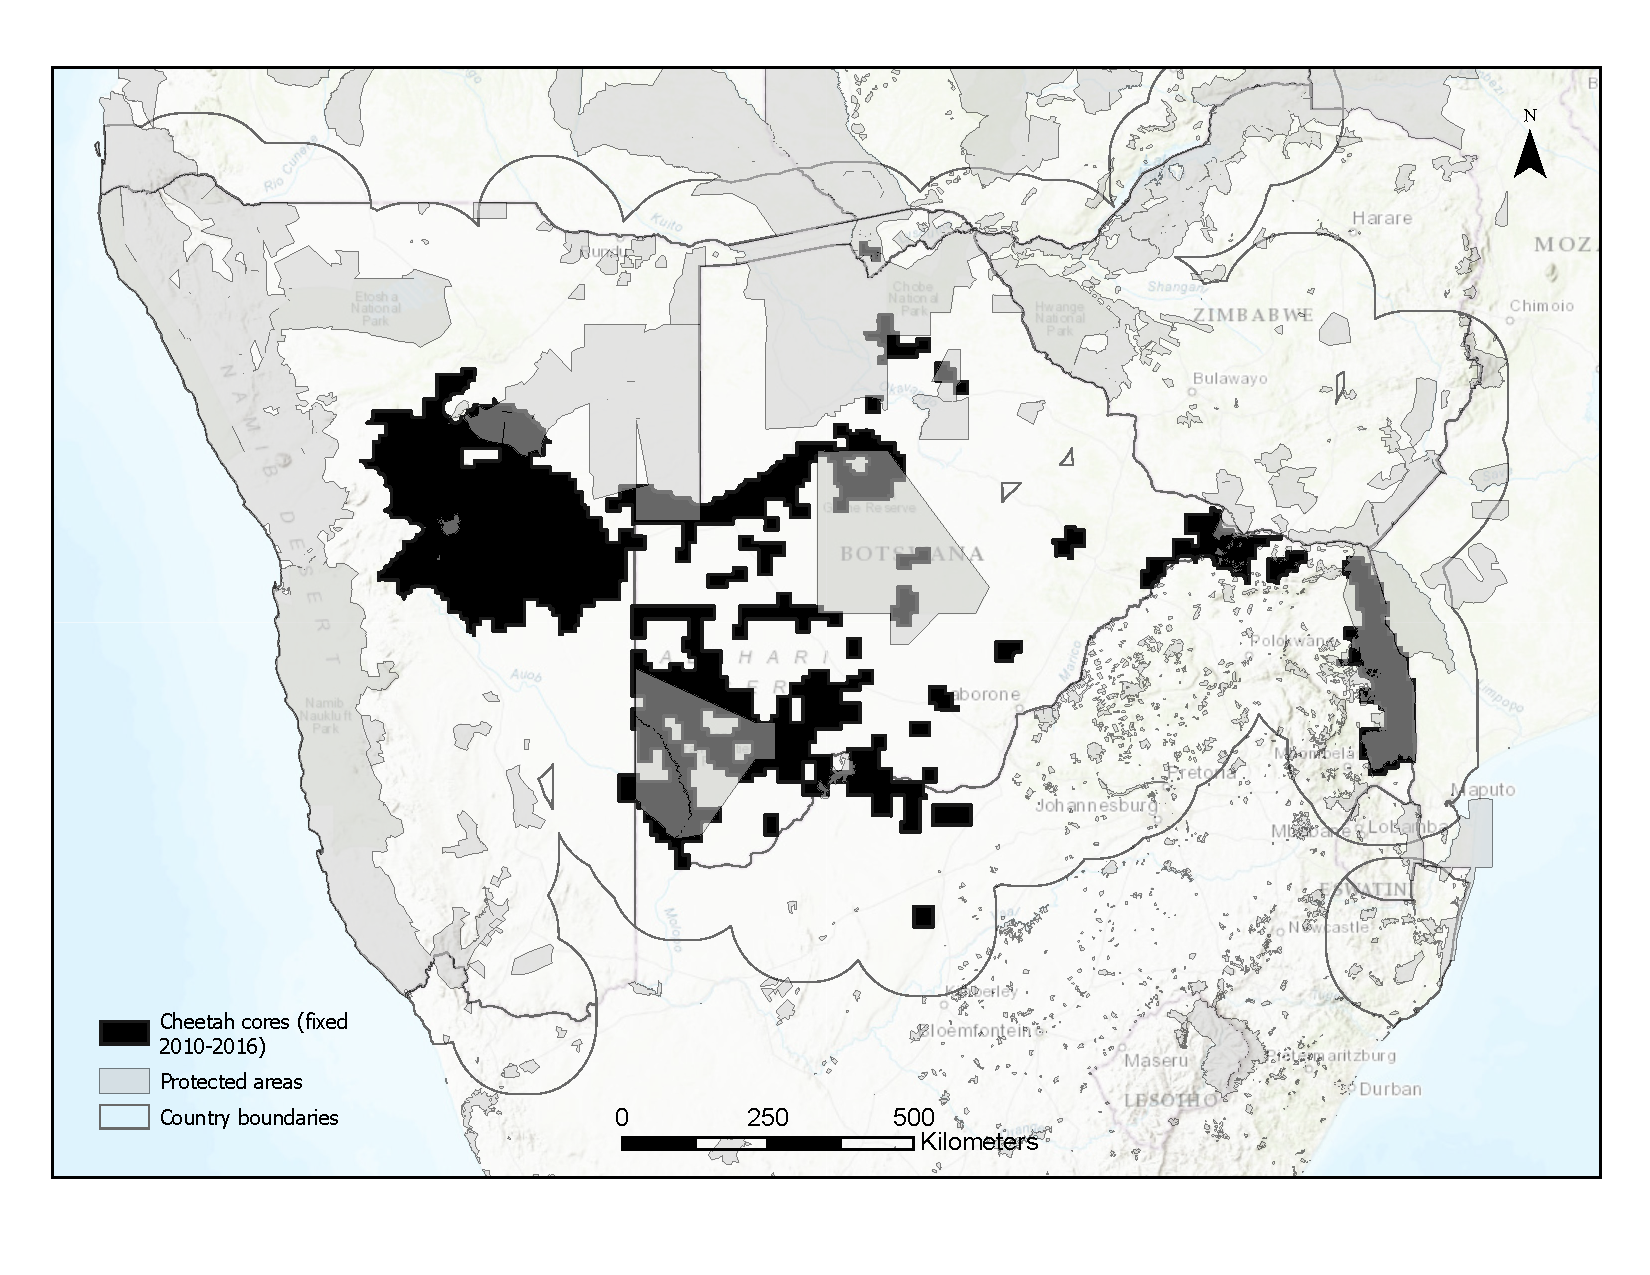
\includegraphics[width=\textwidth]{Figure_0_study_area_and_core_groups.pdf}
  \caption{Study extent, fixed historical range cores, and core groups used to define
  the modeled connectivity network. Core groups are an analysis construct and do not
  imply separate populations.}
  \label{fig:studyarea}
\end{figure}

\subsection{Range cores}
\label{sec:cores}

I defined a core area as a contiguous patch of cells that were confirmed presence, with a density of $\geq$ 0.51 cheetahs per 100~km$^2$, which was from the density raster's own natural breaks that represent the core areas best \parencite{weise2017data}. The final network consisted of 23 cores, which were held constant across all four temporal snapshots to avoid inventing core movement in the absence of comparable range reassessment. The minimum for the core size was 500~km$^2$ based on an average of observed ranges per cheetah \parencite{melzheimer2020hubs}.

I represented these 23 core areas as fixed nodes across all four temporal snapshots (2012, 2016, 2020 and 2024). I took each core area and calculated the Euclidean distance to the three nearest neighbors and a minimum spanning tree was added to ensure all cores were connected. This yielded 45 straight-line links. These straight-line links defined the lines used to get the least cost paths based on the added resistance surface rasters (\ref{sec:graph}).

\subsection{Covariates and their temporal treatment}
\label{sec:covariates}

The predicted temporal resistance values came from the continuous rasters (human development from GHSL, nighttime lights from VIIRS, and VCF (vegetation) from MODIS). Categorical land cover was used for masking and description only, because annual categorical features can switch classes between years for reasons unrelated to overall landscape change.

I also used the static covariates (roads, livestock, terrain, hydrography, fences, protected areas, and core definitions). The static covariates did not contribute \textit{temporal} signal to the resistance surface; however, they did contribute \textit{spatial} signal to the resistance surface. The static covariates were used to describe the landscape and to provide context for the dynamic covariates.

\TODO{TABLE (moved here from Results, 6 October 2026): mention the covariates table in this subsection, e.g. ``(Table\textasciitilde\texttt{\textbackslash ref\{tab:covariates\}})'' after you first list the covariates. It is now the first table in the paper. The gaps in the table itself are listed in the note under it.}

\begin{table}[htbp]\centering
  \caption{Input layers, their data sources, how each was treated through time, and whether it entered the resistance surface.}
  \label{tab:covariates}
  \small\begin{tabular}{>{\raggedright\arraybackslash}p{0.22\textwidth}>{\raggedright\arraybackslash}p{0.24\textwidth}>{\raggedright\arraybackslash}p{0.13\textwidth}>{\raggedright\arraybackslash}p{0.34\textwidth}}
\toprule
Covariate & Source & Treatment & Temporal role / notes\\
\midrule
Built-up fraction & Global Human Settlement Layer (GHSL) & Dynamic & 2010, 2015, 2020, 2025 products matched to snapshots\\
Nighttime radiance & Visible Infrared Imaging Radiometer Suite (VIIRS), VNL V2 & Dynamic & 2013, 2016, 2020, 2024 products\\
Tree cover & Moderate Resolution Imaging Spectroradiometer (MODIS), MOD44B & Dynamic & Annual snapshot fields\\
Non-tree vegetation & Moderate Resolution Imaging Spectroradiometer (MODIS), MOD44B & Dynamic & Annual snapshot fields\\
Bare cover & Moderate Resolution Imaging Spectroradiometer (MODIS), MOD44B & Dynamic & Annual snapshot fields\\
Road density & Global Roads Inventory Project, version 4 (GRIP4) & Static & Spatial pressure/context\\
Livestock density & Gridded Livestock of the World, version 4 (GLW4) & Static & Combined cattle, goats, and sheep exposure\\
Terrain / slope & Shuttle Radar Topography Mission (SRTM) & Static & Slope-derived resistance\\
Hydrography & Hydrological data and maps based on Shuttle Elevation Derivatives at multiple Scales (HydroSHEDS) & Static & Water/context mask\\
Veterinary fences & World Wide Fund for Nature (WWF), Kavango--Zambezi Transfrontier Conservation Area (KAZA); Kruger references & Scenario & Sensitivity/context, not assumed impassable\\
\bottomrule
\end{tabular}
\\[0.5em]
\parbox{\textwidth}{\footnotesize\emph{Note:} Product shorthand retained in the source names is defined at first use: VNL = VIIRS nighttime lights; V2 = product version 2; MOD44B = MODIS vegetation-continuous-fields product.}
\\[0.5em]
\noindent\TODO{THREE GAPS IN THIS TABLE, in plain terms.\\
1. The reader cannot tell which layers actually went into the resistance surface. Your final model used built-up, roads, livestock, and nighttime lights (human pressure), vegetation, and slope. Hydrography is listed as ``Water/context mask,'' but it was not one of the weighted inputs. Add a column or a note saying ``in resistance: yes/no'' so nobody assumes water was a barrier.\\
2. Categorical land cover (MCD12Q1) is not listed, but Methods says it was used for masking and description. Add it as ``Context only, never differenced.''\\
3. Protected areas (WDPA, August 2026) are not listed, but they drive a whole Results section. Add them as ``Overlay for reporting only, not a resistance input.''}

\end{table}

\subsection{Resistance scenarios}
\label{sec:resistance}

Resistance values were assigned to represent the relative difficulty of movement through each landscape feature. The terrain component was derived from slope, with steeper slopes assigned higher resistance values. The final balanced map had a weight of 60\% for human pressure, 20\% for vegetation, and 20\% for terrain. Within human pressure, built-up land, roads, and livestock each received 30\%, while nighttime lights received 10\%. Available fence data was incorporated into the resistance model, with fence cells increasing the combined resistance by a multiplier of 1 if there is no fence, or 25 if there is a fence cell. Fences did not incur a full block to cheetah movement as they are not complete barriers \parencite{cozzi2013barriers}. I treated slopes near 15 percent as easiest for movement and assigned more resistance above or below that point. This had to be done carefully however, given cheetahs do have an affinity for some sloped terrains \parencite{moqanaki2017iran}. I compared alternative vegetation weights because vegetation cover can influence cheetah habitat use \parencite{verschueren2024guild}. Different weighting schemes allowed me to test how strongly the modeled resistance surfaces depended on the vegetation weight \parencite{zeller2012resistance}. The final resistance surface was used to model least-cost paths and Circuitscape current flow between core areas.

\TODO{RESISTANCE PARAGRAPH, FOUR FIXES.\\
1. SLOPE IS DESCRIBED WRONG. The paragraph says steeper slopes cost more, then says slopes near 15 percent are easiest with resistance rising above AND below. The code (\texttt{create\_terrain\_resistance.py}) does neither of the second thing: slopes of 10 DEGREES or less get resistance 1, resistance rises in a straight line to 10 at 30 degrees, and anything steeper stays at 10. Flat ground is easiest and there is no sweet spot. Note the unit is degrees, not percent, and slope is the average within each 1-km cell. Rewrite to match, and drop the ``affinity for sloped terrain'' line unless it supports the 10-degree free zone.\\
2. SAY WHO CHOSE THE NUMBERS. The 60/20/20 split, the 30/30/30/10 split inside human pressure, the 10-to-30-degree slope ramp, and the times-25 fence multiplier were your choices, informed by the papers you cite. None were fitted to cheetah movement data. Say that in one plain sentence. Reviewers accept chosen values; what they do not accept is values that look fitted when they were not.\\
3. LIST WHAT ELSE WAS RUN. Name every alternative so \texttt{\textbackslash nscen} can be filled in: three human-pressure weightings (your main one, equal, and infrastructure-emphasis), three vegetation weights (10, 20, and 40 percent), and the fence treatments (no fences, documented fences, near-barrier, Kruger documented, and Kruger conservative). Careful when counting: your main surface is one member of each list, so it is a main surface plus 8 alternatives, not 11.\\
4. THE ``PRIMARY'' SURFACE IS A CHANGE FROM THE PLAN. Your protocol said no scenario would be treated as the main answer. The paper uses the vegetation-balanced surface with documented fences as the main one. That is a reasonable choice, but it needs one sentence here explaining why, and a line in Appendix A1.}

\subsection{Connectivity modelling}
\label{sec:connectivity}

For each core, I ran a least-cost analysis in ArcGIS, which calculated the accumulated cost of moving through every reachable cell. I then used the lowest accumulated cost to draw paths from the starting core to each connected destination. Reusing the accumulated-cost calculation for several destinations produced the same set of pairwise paths with fewer repeat calculations. I also used Circuitscape 5.17.1 to model the distribution of possible movement routes between each pair of cores. The analysis included all 253 core pairs in each of the four years, for a total of 1,012 pairwise comparisons.

\subsection{Network structure}
\label{sec:graph}
\TODO{PLAIN-LANGUAGE WRITING GUIDE.
What was measured: edge betweenness counts how often a link lies on the shortest
network route between pairs of cores. A high value means the link helps hold many parts
of the modeled network together. The value was calculated on the 45-link network and
divided by the 253 possible core pairs.
How links were chosen: the network combined each core's three nearest neighbors with
a minimum spanning tree, which is the smallest set of links needed to keep the core
network connected.
Why rankings are uncertain: allowing two, three, four, or five nearest neighbors
created 31, 45, 61, or 77 links, and the highest-ranked links changed. Link 17--24 was
the only bridge under the three-neighbor choice; removing a bridge separates the
network into two pieces.
What was dropped: PC and dPC \parencite{saura2007pc} require an assumed relationship
between distance and dispersal. No local dispersal telemetry was available, so those
more detailed-looking numbers were not calculated. Cite \textcite{keeley2021metrics}
when explaining that the metric should match the research question.\\
FIX THE REASON ABOVE BEFORE YOU WRITE IT. ``No dispersal telemetry'' was already known when the protocol was locked, and the protocol handled it: decision 4 set 100~km as the dispersal value, based on how far apart cheetah communication hubs are \parencite{melzheimer2020hubs}, with 50, 200, and 400~km as checks. So that cannot be the reason PC was dropped; a reader comparing the protocol would spot it. Write down the real reason. It might be that betweenness answers H1 directly and PC would add a second ranking to explain, or that a single borrowed 100~km value would make the numbers look more precise than they are. Whatever it was, say it plainly, and add it to Appendix A1 as a change from the plan.}

\subsection{Temporal comparison}
\label{sec:temporal}
\TODO{PLAIN-LANGUAGE WRITING GUIDE: compare the same core pairs, model assumptions,
and 1-km grid in 2012, 2016, 2020, and 2024. This keeps the comparison consistent so
the modeled differences come from the input layers that changed through time. Define
absolute change as later value minus earlier value. Define percent change as that
difference divided by the earlier value, multiplied by 100.}


\subsection{Protected-area coverage}
\label{sec:pa}
\TODO{PLAIN-LANGUAGE WRITING GUIDE.
Question: what share of the modeled connecting landscape outside the cores falls inside
protected areas?
Data preparation: use the August 2026 WDPA release
\parencite{unepwcmc2026wdpa}. Keep terrestrial and coastal protected-area polygons,
remove proposed areas, points, and marine-only areas, and merge overlaps. This left
2,301 records in the study extent.
Comparison area: 31.26 percent of the usable outside-core area was protected. Cells
with zero current were excluded because they could never enter a high-current group.
Why no p-value: the answer changed from significant to not significant when the
assumed spatial block size changed. Report the descriptive percentages and note that
the same general pattern appeared in all four years and under several core-buffer
sizes.}

\subsection{Stability and uncertainty}
\label{sec:uncertainty}
\TODO{PLAIN-LANGUAGE WRITING GUIDE.
What "stable" means here: a link had to pass three checks. First, both alternative
weightings had to keep at least 80 percent of the route within 5 km of the main route;
34 of 45 passed. Second, the fence scenarios could not substantially change the link;
this removed two more from the group. Third, the direction of change had to stay the
same under all vegetation weightings. The two links that failed this last check had
already been removed. The final groups were 32 main-priority links and 13 uncertain
links.
Important distinction: the 80-percent-within-5-km rule is not the cell-by-cell agreement
test proposed in the original protocol, even though both use the number 80 percent.
What was not completed: alternative core definitions, 2-km and 5-km grids, and a
cell-by-cell agreement map.
Separate location uncertainty from cost uncertainty: 49 of 180 route-and-year
comparisons had less than 80 percent overlap within 1 km, including 21 main-priority
links. Link 17--24 had no overlap in 2020. This does not mean the connection was
unimportant; it means the exact mapped route was uncertain.}

\subsection{Independent plausibility assessment}
\label{sec:validation}
\TODO{PLAIN-LANGUAGE WRITING GUIDE. UPDATED 5 OCTOBER 2026: THE PLANNED CHECK IS NOW DONE.\\
Never call this ``validation.'' No resistance value was fitted to these tracks, so it is a plausibility check: does the model's picture of easy and hard land line up with where real cheetahs spent their time?\\[0.3em]
DATA: tracking data from nine free-roaming cheetahs (seven males, two females) collared near Thabazimbi, Limpopo, South Africa, from September 2003 to November 2008 by the Endangered Wildlife Trust and the University of Pretoria. Cite the dataset parencite{marnewick2017ewtdata} and the paper that describes the collaring parencite{marnewick2017tracking}. License CC-BY 4.0, so citing is all that is required. It is independent of your cores, and you can say why in one sentence: these collar locations are not in the Dryad range archive the cores were built from. I checked. The archive's 458 Endangered Wildlife Trust rows are 2014--2015 tourist sightings, not these collars, and only four archive records of any kind fall inside the area these cheetahs used (three farmer questionnaires and one sighting, 2012--2015). That also explains why no core sits in this area.\\[0.3em]
STEPS, matching protocol steps 23.1 to 23.5:\\
1. Downloaded all 3,165 locations. Dropped 17 that had no full date.\\
2. Kept one location per animal per day (the earliest fix) so a single busy collar could not dominate. This left 1,006 locations. One collar alone had 1,954 of the raw fixes, which is why this step matters.\\
3. Made ten random ``available'' points per cheetah location (10,060 in total), spread evenly inside the smallest shape that encloses all the cheetah locations. This asks: within the landscape these animals actually used, did they favor the places the model calls easy? Repeated with that shape widened by 20~km to check the answer did not depend on where the edge was drawn.\\
4. Read the modeled resistance and current at every point, using the 2012 surfaces because the tracks are from 2003--2008, the closest snapshot.\\
5. Compared the two groups, and repeated everything on your earlier model (pressure and terrain only, no vegetation, no fences).\\[0.3em]
ADDED AFTER THE PLAN (5 OCTOBER 2026), FOUR STRICTER FOLLOW-UPS. Say in one sentence that these go beyond the protocol and were added because steps 3 to 5 have two weak spots: they treat a thousand daily locations as independent when the real sample is nine animals, and comparing against the whole area only shows that the animals' home ground was easier, not that they chose easier ground.\\
6. STEP CHECK (the main tracking result now). Took every pair of locations from the same animal on back-to-back days that were at least 1~km apart (549 moves; 303 shorter moves stayed in the same 1~km cell and 145 pairs had a gap of more than a day). For each real move, made 20 moves the same cheetah could have made instead: same starting point, a step length drawn from that animal's own moves, random direction. Then asked what share of those 20 the real move beat (lower resistance, higher current), at the end point and averaged along the straight line. 0.50 means no difference. Each animal gets one score, and the 95\% interval comes from resampling the nine animals 10,000 times, so the animal is the unit, not the location. This design is borrowed from step-selection studies; cite it with parencite{fortin2005wolves, thurfjell2014ssf} (Fortin introduced the matched ``could have gone instead'' design; Thurfjell is the standard review of it). Both are in the bib.\\
7. LAYER BREAKDOWN. Rebuilt the main 2012 surface from its parts, using the same scaling and weights as the build scripts (it matched the stored surface at 99.97\% of sampled points). Scored each part on its own, then scored the main surface with each part left out. This shows which inputs carry the result. Say clearly that nothing was reweighted afterward; this is a description, not a tuning step.\\
8. ALL NINE SURFACES. Repeated the step check on the main surface and the eight alternatives. This tests whether the result depends on one set of assumptions. Say it was not used to choose a surface.\\
9. ROAD CROSSINGS. Counted how often real moves crossed a mapped GRIP4 road compared with the alternative moves. Fences could not be tested this way: no mapped fence lies within 20~km of any track.\\[0.3em]
THINGS TO STATE OPENLY: the tracks end four years before your first snapshot; nine animals in one district cannot speak for the whole network; none of the locations fell inside a core, so the current values are not inflated by the cores; the straight line between two daily locations is not the route the animal walked; and the fence part of the model is untested by these data. Scripts in the connectivity repo: \texttt{analysis/scripts/plausibility\_limpopo\_tracks.py} (steps 1 to 5), \texttt{plausibility\_limpopo\_steps.py} (step 6), and \texttt{plausibility\_limpopo\_followups.py} (steps 7 to 9).\\[0.3em]
THE OLD SAME-ARCHIVE CHECK: keep it, but as a second, weaker check, and say it is not independent because it uses the records that built the cores. Numbers: after thinning to one record per 10-km cell, 2010--2012 had 413 cells and 2013--2016 had 450, with an overlap score of 0.239. There are no records after 2016.\\[0.3em]
STILL NOT DONE: the central-eastern Namibia camera-trap comparison \parencite{verschueren2024guild}. Those data are request-only. Either request them or state in one sentence that this second planned source was not obtained.}

All inputs to the connectivity model are static. The cores are fixed from historical records, the landscape is represented by four snapshots, and the modeled paths are estimates rather than observed routes. To assess whether this static representation bears any relation to how cheetahs actually move, the model was compared with independent GPS tracking data from free-ranging cheetahs. This comparison is a plausibility check rather than a validation, because no resistance value was fitted to these data. The tracking data consist of 3,165 locations from nine free-ranging cheetahs (seven males and two females) collared near Thabazimbi, Limpopo Province, South Africa, between September 2003 and November 2008 \parencite{marnewick2017ewtdata, marnewick2017tracking}. The tracked area lies inside the study extent but outside every core, so these animals were moving through the landscape between cores, which is the part of the map the model makes claims about. The data are also independent of the cores, as none of these collar locations appear in the range archive from which the cores were derived \parencite{weise2017data}.

Seventeen records without a complete date were removed, and the remaining locations were thinned to the earliest fix per animal per calendar day, leaving 1,006 locations. Locations from the same animal on consecutive days were then paired into day-to-day moves. Moves shorter than 1~km were excluded because both ends fall within the same 1~km cell, which left 549 moves with a median length of approximately 4~km. Each move was compared with 20 alternative moves the same animal could have made instead, following the logic of step-selection analysis, a method that compares observed movements with the alternatives available from the same starting point \parencite{fortin2005wolves, thurfjell2014ssf}. Each alternative began at the same location as the real move, covered a distance drawn from that animal's own movements, and headed in a random direction. Because every alternative began where the real move began, the comparison reflects the animal's choice of destination rather than the general character of the area it lived in. Modeled resistance was read from the 2012 surfaces, the snapshot closest to the tracking period, at the end point of each move and averaged along the straight line between its start and end. For each move, the share of alternatives that reached higher resistance than the real move was recorded. If modeled resistance had no bearing on movement, this share would be approximately 0.50. Shares were averaged within each animal so that each of the nine animals counted once, and a 95\% interval was derived by resampling the animals 10,000 times.

\TODO{Co-written 5 October 2026 from your answers. Still to add, one or two sentences each: the broader comparison against random points across the whole tracked area (steps 3 to 5 in the guide above), the layer breakdown, the repeat on all nine surfaces, and the road-crossing count.}

\subsection{Monitoring prioritisation}
\label{sec:mcda}
\TODO{PLAIN-LANGUAGE WRITING GUIDE.
What was planned: combine six measurements into one score for every 10-km cell and
test three sets of weights.
What was built instead: a link-level table that keeps each kind of evidence separate.
Its columns describe how important the link is to the network, how its modeled cost
changed, how stable its mapped route was, whether fences affected it, and how much of
it is protected.
Why this is more honest: combining everything into one score would require deciding,
for example, how much route instability is equal to a change in protection. No
evidence-based exchange rate was available. State clearly that no combined monitoring
score was calculated.} There is a cheeta \TODO{Unfinished sentence fragment left here; finish or delete it.}

\subsection{Software and reproducibility}
\label{sec:software}
\TODO{PLAIN-LANGUAGE WRITING GUIDE: list the software without explaining every
technical setting in the main text. Verified versions are ArcGIS Pro
\arcgisversion\ (build \arcgisbuild), ArcGIS Python \pythonversion, Julia
\juliaversion, and Circuitscape.jl \circuitscapeversion; point readers to the full
software table in \suppB. Google Earth Engine supplied and aligned the satellite data.
Most ArcGIS processing used Python scripts rather than ModelBuilder. Add the final
archive link and state which source datasets cannot legally be redistributed.\\[0.3em]
AI DISCLOSURE, REQUIRED BY BIODIVERSITY AND CONSERVATION. The journal says use of a
large language model ``should be properly documented in the Methods section,'' unless
it was only used for copy editing (grammar, spelling, readability). You used an AI
assistant for more than that: writing and debugging analysis scripts, building the
tracking-check scripts, checking numbers against the source files, and drafting
writing guides and some text that you then revised. Add one or two honest sentences
here, for example: ``An AI assistant (Claude, Anthropic) was used to help write and
debug analysis scripts and to draft text, which the author reviewed, revised, and
verified against the source outputs. The author takes full responsibility for the
content.'' AI tools cannot be listed as an author. The capstone may have its own rule
on AI use, so check that with your advisor too.}

\section{Results}
\label{sec:results}

% Results report numbers. No mechanism, no conservation implication, no
% "suggesting that". Every one of those belongs in the Discussion.

\subsection{Connectivity change, \studyperiod}
\TODO{PLAIN-LANGUAGE WRITING GUIDE.
What happened: I compared all 253 possible pairs of cores. Overall, the modeled cost
of moving between cores changed only a little from 2012 to 2024. The middle change was
-1.224 percent. A negative value means the model became slightly easier to move
through; it does not mean that cheetahs actually moved more. Of the 253 pairs, 92
became harder and 161 became easier. The largest increase was +13.1 percent for the
link between cores 33 and 38.
What the map adds: outside the cores, the places with the highest modeled current were
mostly in the same locations through time. Their overlap scores were 0.91 to 0.93,
where 1 would mean perfect overlap.
What not to claim: do not call this an overall connectivity loss, observed movement,
or a country-by-country result. The analysis did not assign each core pair to a
country. For H1, report that 18 of the 45 selected links became harder and 27 became
easier, but that change was not meaningfully related to baseline betweenness
($\rho \approx 0.01$). Therefore H1 was mixed rather than supported. Use
\figref{fig:change}. When you point to a figure in your own sentences, type
\texttt{\textbackslash figref\{fig:change\}} rather than ``Figure'' by hand: it prints
``Figure'' in the capstone and ``Fig.'' in the journal layouts, which is how Springer writes it.\\
H1, TWO MORE NUMBERS YOU CAN USE (checked 5 October 2026; same answer, stated the way the protocol worded H1). The $\rho \approx 0.01$ above mixes the links that got harder with the ones that got easier. Asking the protocol's question directly: (1) Did the 18 harder links have higher betweenness than the 27 easier ones? Slightly, but not meaningfully (Mann--Whitney one-sided $p = 0.36$). (2) Among the 18 harder links, did the bigger losses fall on the more important links? No; if anything the reverse ($\rho = -0.22$, not significant). One thing that DID match: the losses were fairly concentrated, with the 5 hardest-hit of the 18 links carrying 46 percent of the total increase. So H1's ``minority of links'' half holds, and its ``high-betweenness links'' half does not.\\
FIGURE PLACEMENT: the study-area figure just below shows the extent and cores, which is setup, not a result. Move it to Methods, near Study area.}

\begin{figure}[htbp]\centering
  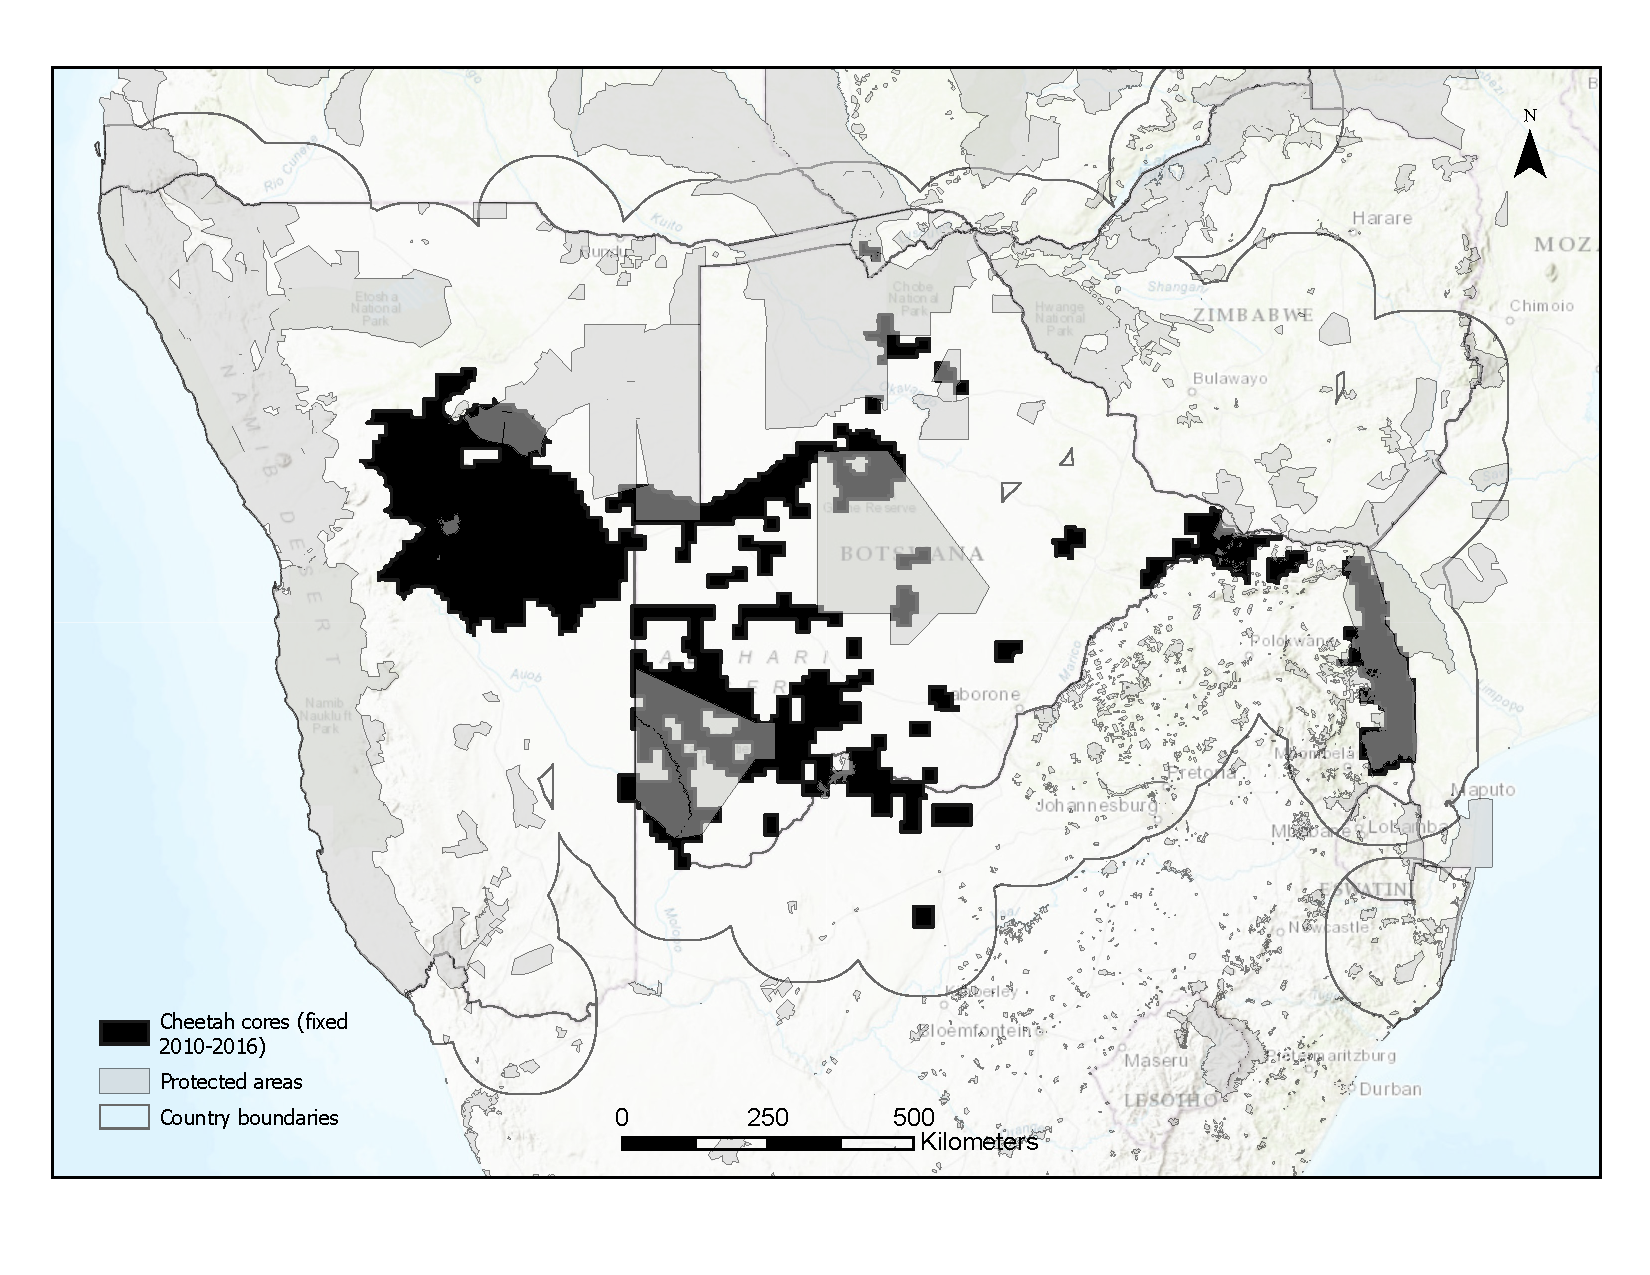
\includegraphics[width=\textwidth]{Figure_0_study_area_and_core_groups.pdf}
  \caption{Study extent, fixed historical range cores, and core groups used to define
  the modeled connectivity network. Core groups are an analysis construct and do not
  imply separate populations.}
  \label{fig:studyarea}
\end{figure}
\FloatBarrier

\subsection{Priority links and sensitivity checks}
\TODO{PLAIN-LANGUAGE WRITING GUIDE.
What happened: 32 of the 45 selected links passed the tested sensitivity screens
and remained in the main priority group. Network importance was ranked separately
using betweenness. The other 13 links were kept as
uncertain links where more field information would be useful. The weighting test kept
34 links, and the fence test removed two more. The vegetation test did not remove any
additional links from the remaining group.
What it means: the main group is not a small handful of links; it contains most of the
network. That only partly matches the original expectation that priorities would be
limited to a small subset.
What not to claim: these links are modeled connections between cores, not confirmed
animal travel routes. Use Table~\ref{tab:top20}.}

\begin{figure}[htbp]\centering
  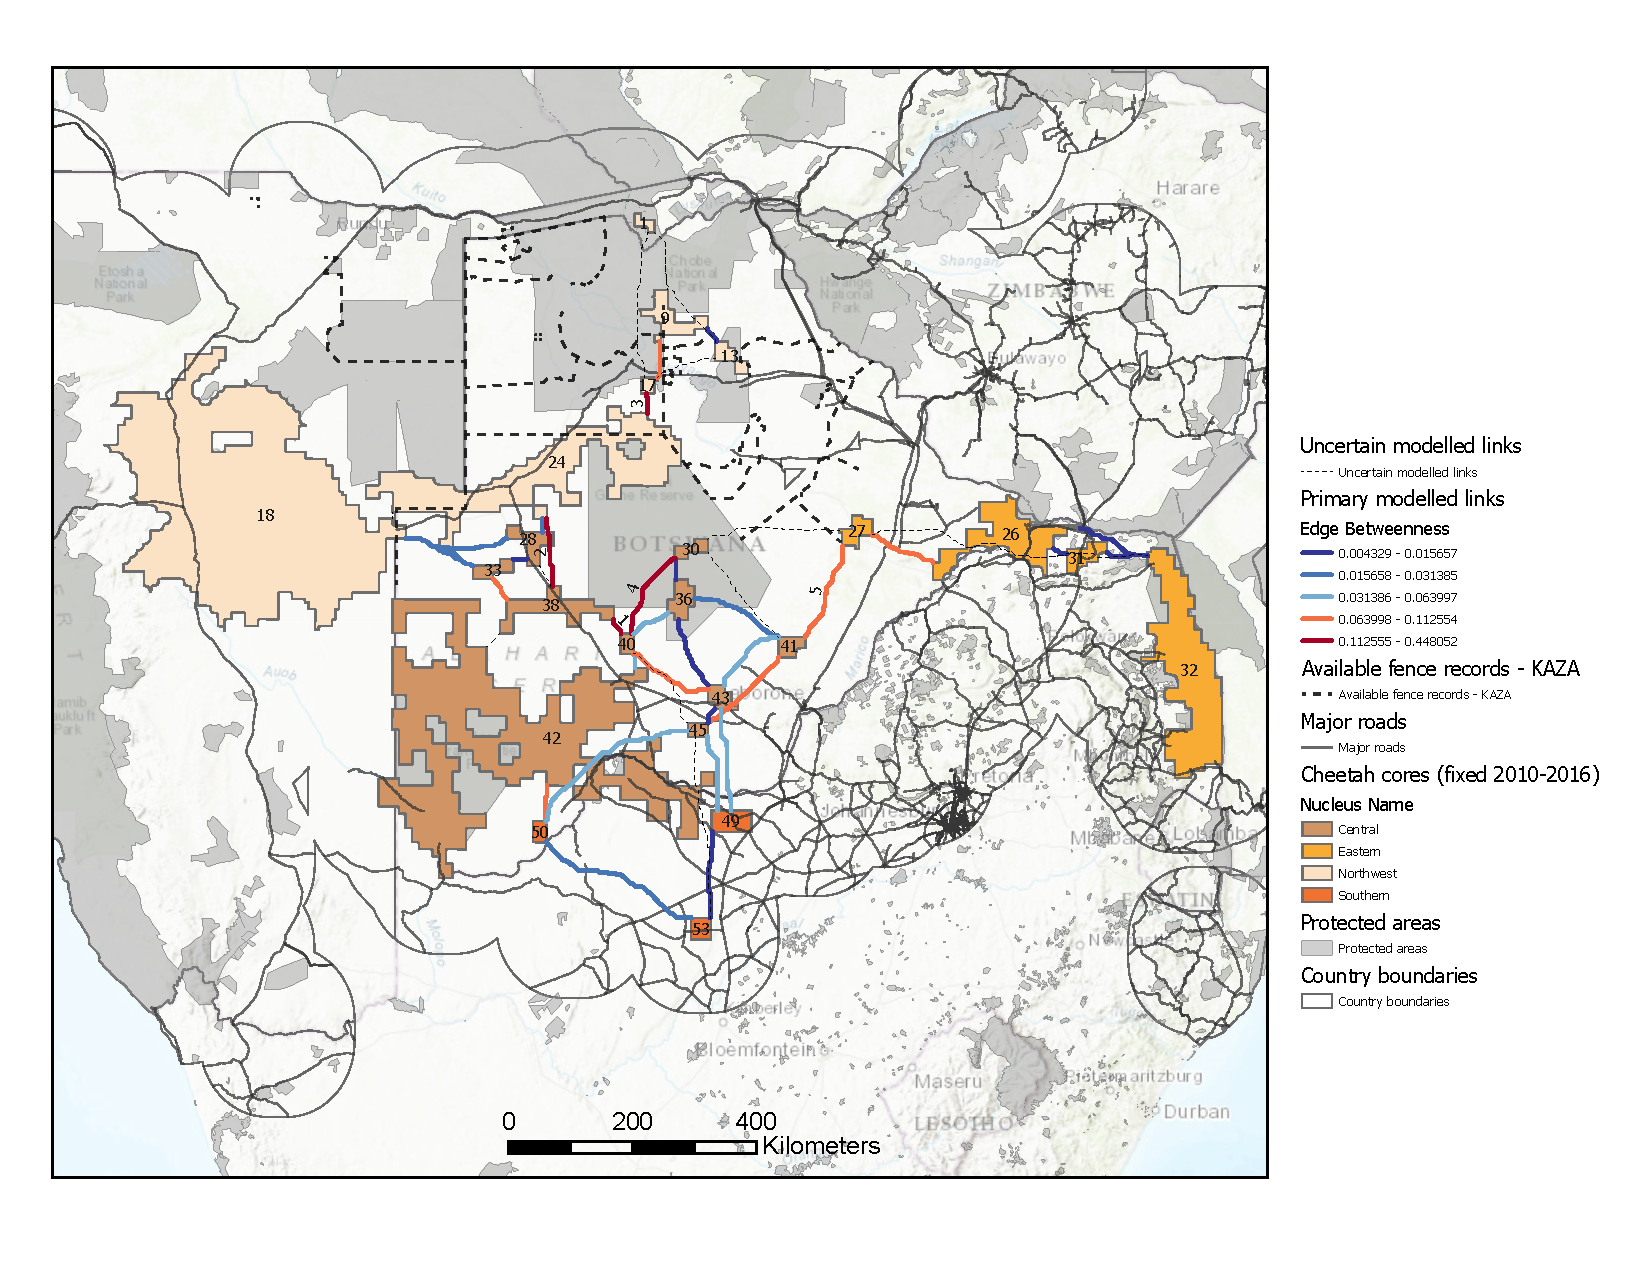
\includegraphics[width=\textwidth]{Figure_5_modelled_links_and_transportation.pdf}
  \caption{Modeled core-to-core links with transportation and available fence context.
  Lines represent network links used to define least-cost analyses; they are not
  observed animal paths.}
  \label{fig:networkcontext}
\end{figure}
\FloatBarrier

% Sensitivity evidence explains the priority-link screening above.
\TODO{PLAIN-LANGUAGE WRITING GUIDE FOR THE SENSITIVITY TESTS.
Main lesson: the total modeled cost of a connection was usually fairly stable, but
the exact line taken by the least-cost path was less stable. Of 180 route-and-year
comparisons, 49 had less than 80 percent overlap within 1 km. This affected 21 of the
32 priority links. The route between cores 17 and 24 had no overlap in 2020.
Vegetation assumptions: 43 of 45 links kept the same direction of change under all
three vegetation weightings. However, the size of the change grew as vegetation was
given more weight: the middle absolute change increased from about 3.6 to 9.3 percent.
Network-design assumption: changing how many neighbors each core could connect to
changed the number of links and changed which links ranked highest. A bridge is a link
whose removal splits the network into separate pieces; link 17--24 was the only bridge
when three nearest neighbors were used.
What not to claim: there is no completed cell-by-cell agreement map, and no single
ranking should be presented as certain. State that H3 was only partly evaluated: a
 stable group existed, but it contained a majority of the selected links and the full
planned sensitivity grid was not completed.}

\TODO{PLAIN-LANGUAGE WRITING GUIDE FOR THE INDEPENDENT TRACKING CHECK (UPDATED 5 OCTOBER 2026 WITH THE STRICTER FOLLOW-UPS).\\
Give this its own short subsection; it answers a different question from the priority links. Numbers only here; meaning goes in Discussion. Lead with the step check (Table~\ref{tab:limpopo_steps}), because it is the stricter test. Put the first comparison (Table~\ref{tab:limpopo}) after it as background, or move that table to \suppB.\\[0.3em]
1. THE MAIN RESULT (Table~\ref{tab:limpopo_steps}, panel A). Across 549 day-to-day moves, the place a cheetah actually went had lower modeled resistance than the moves it could have made instead. The real move beat 56 percent of its alternatives (95 percent interval 51 to 61 percent), where 50 would mean no difference, and seven of the nine animals leaned that way. Averaged along the straight line between locations the result was almost the same (55 percent).\\
2. CURRENT DID NOT HOLD UP. The real move beat 53 percent of alternatives on modeled current, but the interval (47 to 59) includes 50, and only five of nine animals leaned that way. Say this plainly. It also means the 65 percent for current in the first comparison mostly reflected where the cats lived, not the choices they made each day.\\
3. ALL NINE SURFACES (panel B). Every surface gave 55 to 56 percent, so the result does not depend on which weighting you picked. The four other fence treatments give exactly the same values as the main surface because no mapped fence lies within 20~km of any track.\\
4. WHICH LAYERS CARRY IT (panel C). Road density did most of the work: on its own it reached 55 percent, about as much as the full surface, and leaving it out dropped the full surface to 54 percent with an interval that just touches 50. Livestock, slope, and night lights each added a small lean (51 to 52 percent). Built-up area did nothing here because there is almost none in this district. Vegetation on its own leaned slightly the wrong way (48 percent, interval 43 to 52, which includes 50). Report that honestly; do not hide it.\\
5. ROAD CROSSINGS (panel D). 26 percent of real moves crossed a mapped road, against 35 percent of the alternatives; eight of nine animals crossed less than expected. Major roads were crossed too rarely by anyone (1 against 2 percent) to say much.\\
6. THE FIRST COMPARISON (Table~\ref{tab:limpopo}), as background: against random points across the whole area, cheetah locations had lower resistance 60 percent of the time (7 of 9 animals) and higher current 65 percent of the time (6 of 9). Widening the area by 20~km and using the earlier model gave the same picture.\\[0.3em]
HOW TO DESCRIBE THE STRENGTH: consistent in direction, modest in size, and mostly carried by roads. 56 percent is a real lean, not a strong one. Say ``consistent with'' the model, not ``confirmed.'' Report the intervals and animal counts, not p-values.\\[0.3em]
WHAT NOT TO CLAIM: that the model is validated; that it works across the whole region (one district in South Africa); that it says anything about 2020 or 2024 (the tracks end in 2008); or that fences were tested (they were not).}

\begin{table}[htbp]\centering
  \caption{\TODO{Final caption, in your own words: day-to-day moves of nine free-roaming cheetahs (Limpopo, 2003--2008) compared with moves of the same length the animals could have made instead, on the 2012 surfaces. Panels: main surface, all nine surfaces, single input layers, road crossings.}}
  \label{tab:limpopo_steps}
  \resizebox{\textwidth}{!}{\begin{tabular}{llrcr}
\toprule
 & Comparison & Share of alternatives & 95\% interval & Animals \\
 & & the real move beat & (resampling animals) & above 0.50 \\
\midrule
\multicolumn{5}{l}{\textit{A. Main surface, 549 day-to-day moves, 20 alternatives each}}\\
 & Resistance at the end point (lower expected) & 0.56 & 0.51--0.61 & 7 of 9\\
 & Resistance along the straight-line path & 0.55 & 0.51--0.59 & 7 of 9\\
 & Current at the end point (higher expected) & 0.53 & 0.47--0.59 & 5 of 9\\
 & Current along the straight-line path & 0.52 & 0.47--0.58 & 5 of 9\\
\midrule
\multicolumn{5}{l}{\textit{B. All nine surfaces, resistance at the end point}}\\
 & Main surface & 0.56 & 0.51--0.61 & 7 of 9\\
 & Equal human-pressure weights & 0.56 & 0.51--0.61 & 7 of 9\\
 & Infrastructure emphasis & 0.56 & 0.50--0.61 & 6 of 9\\
 & Vegetation weight 10\% & 0.56 & 0.50--0.61 & 7 of 9\\
 & Vegetation weight 40\% & 0.55 & 0.51--0.60 & 6 of 9\\
 & Four other fence treatments$^{a}$ & 0.56 & 0.51--0.61 & 7 of 9\\
\midrule
\multicolumn{5}{l}{\textit{C. Single input layers, resistance at the end point}}\\
 & Road density & 0.55 & 0.50--0.62 & 6 of 9\\
 & Livestock & 0.52 & 0.49--0.56 & 5 of 9\\
 & Terrain (slope) & 0.52 & 0.50--0.54 & 4 of 9\\
 & Night lights & 0.51 & 0.51--0.52 & 8 of 9\\
 & Built-up area$^{b}$ & 0.50 & 0.50--0.50 & 3 of 9\\
 & Vegetation & 0.48 & 0.43--0.52 & 3 of 9\\
 & Main surface without road density & 0.54 & 0.50--0.57 & 7 of 9\\
\midrule
\multicolumn{5}{l}{\textit{D. Road crossings along the straight-line path (fewer expected)}}\\
 & Any mapped road (26\% of real moves crossed, 35\% of alternatives) & 0.54 & 0.52--0.57 & 8 of 9\\
 & Major roads only (1\% against 2\%) & 0.51 & 0.50--0.51 & 5 of 9\\
\bottomrule
\end{tabular}}
\\[0.5em]
\noindent\TODO{Final note, in your own words. Each real day-to-day move (at least 1~km) is compared with 20 moves the same cheetah could have made instead: same start, a step length drawn from that animal's own moves, random direction. The score is the share of those alternatives the real move beat; 0.50 means no difference. Each animal counts once, and the 95\% interval comes from resampling the nine animals. $^{a}$No mapped fence lies within 20~km of any track, so all five fence treatments give identical values here; these data cannot test the fence part of the model. $^{b}$Built-up area barely varies in this district, so it cannot separate real and alternative moves.}

\end{table}

\begin{table}[htbp]\centering
  \caption{\TODO{Final caption, in your own words: modeled resistance and current at
  daily locations of nine free-roaming cheetahs (Limpopo, 2003--2008) compared with
  random available points from the same landscape, on the 2012 surfaces. Call it the broader, less strict comparison.}}
  \label{tab:limpopo}
  \resizebox{\textwidth}{!}{\begin{tabular}{llrrrrr}
\toprule
Surface & Measure & Cheetah fixes & Available & Expected direction & 20-km buffer & Animals\\
 & & (median) & (median) & (share) & (share) & (of 9)\\
\midrule
Final model (vegetation-balanced, documented fences) & Resistance (lower expected) & 2.23 & 2.45 & 0.60 & 0.60 & 7\\
 & Current (higher expected) & 0.156 & 0.145 & 0.65 & 0.62 & 6\\
Earlier model (pressure and terrain only, no fences) & Resistance (lower expected) & 2.03 & 2.34 & 0.61 & 0.61 & --\\
 & Current (higher expected) & 0.143 & 0.128 & 0.65 & 0.63 & --\\
\bottomrule
\end{tabular}}
\\[0.5em]
\noindent\TODO{Final note, in your own words: the comparison uses 1,006 daily locations from nine free-roaming cheetahs (2003--2008) against 10,060 random points from the same landscape, on the 2012 surfaces. ``Expected direction (share)'' is the chance that a random cheetah location had lower resistance (or higher current) than a random available point; 0.50 means no difference. ``20-km buffer'' repeats this with a wider available area. ``Animals'' counts how many of the nine had a median in the expected direction. No location fell inside a core. Add one sentence saying this is the broader comparison, and that in the stricter step check (Table~\ref{tab:limpopo_steps}) the resistance lean held but the current lean did not.}

\end{table}

\TODO{PLAIN-LANGUAGE WRITING GUIDE FOR THE SAME-ARCHIVE OCCURRENCE CHECK.
Keep this, but present it after the tracking check as the weaker of the two, because it is not independent.
What happened: after thinning records to one 10-km cell, the early period had 413
occupied cells and the later period had 450. Their overlap score was 0.239, showing
that the two sets were quite different. Later records occurred in slightly higher
modeled resistance, and a larger share fell inside the fixed cores. Almost no records
were close to the priority paths: zero early cells and three later cells.
Why this is a weak check: the same occurrence archive helped create the cores, so this
is not an independent test. There are also no occurrence records after 2016, so it
cannot check the 2020 or 2024 results. Report it honestly as a limited comparison, not
as validation.}

\TODO{Protocol reporting only: the planned cell-level monitoring index was not built and H4 was not tested. Explain this once in \suppA, not as a repeated priority-link result.}

\subsection{Protected-area coverage of priority connectivity}
\TODO{PLAIN-LANGUAGE WRITING GUIDE.
Why the cores were removed: the model forces current into and out of the cores, so the
cores automatically receive very high current. Including them would make protection
look better without telling us how well the land between cores is protected.
What happened outside the cores: 31.26 percent of the comparison area is protected.
Only 23.27 percent of the area above the 80th current percentile was protected in
2024. Coverage rose to 25.54 percent above the 90th percentile, 33.45 percent above the
95th, and 44.63 percent above the 99th. In simple terms, the very strongest
concentrations often reached protected areas, while the broader connecting landscape
around them was less protected.
What not to claim: do not report a significance p-value because it changed when the
size of the spatial blocks changed. Do not call modeled current observed movement. Use
Table~\ref{tab:pa}. State that H2 was not supported under its full rule because the
direction changed across current thresholds and the significance result was not
stable.}

%------------------------------------------------------------------ figure inserts
\begin{figure}[htbp]\centering
  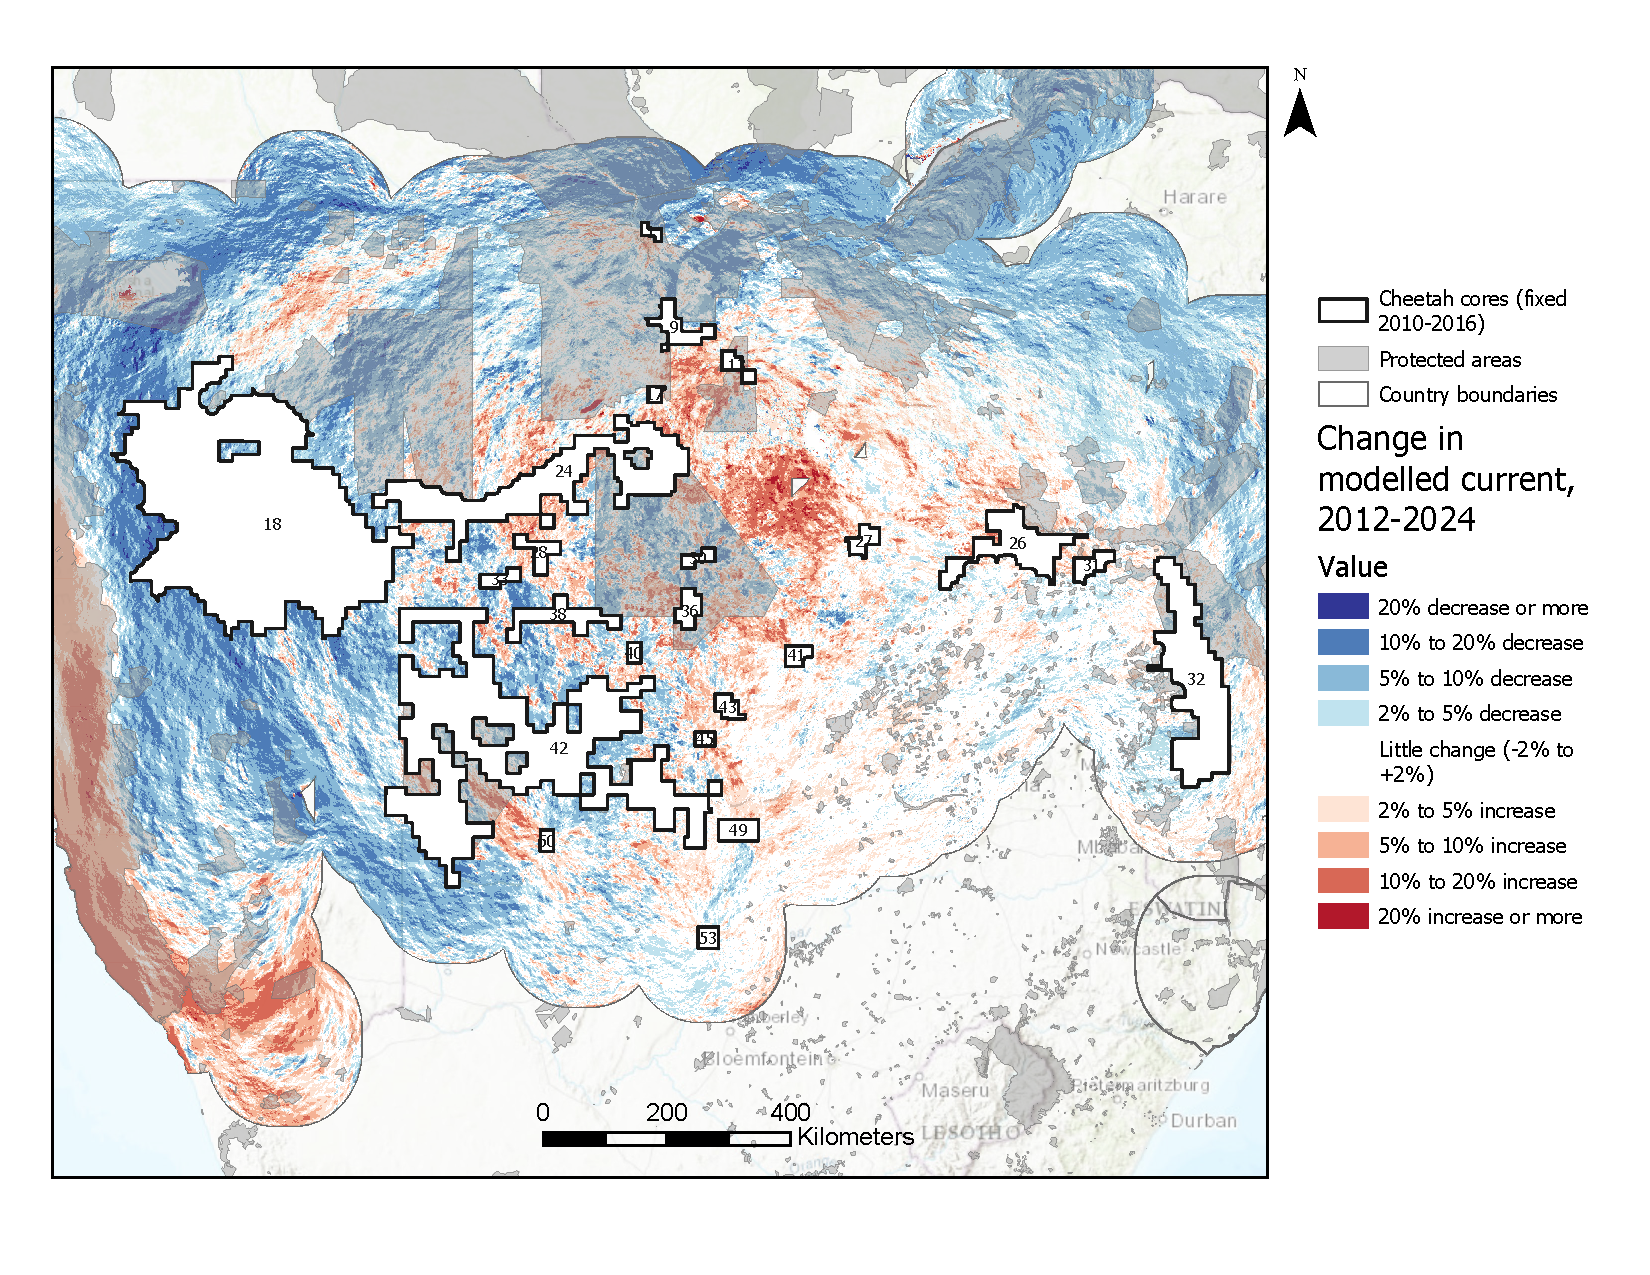
\includegraphics[width=\textwidth]{Figure_2B_current_change_2012_2024.pdf}
  \caption{Modeled current change between 2012 and 2024.}
  \label{fig:change}
\end{figure}
\FloatBarrier

\begin{figure}[htbp]\centering
  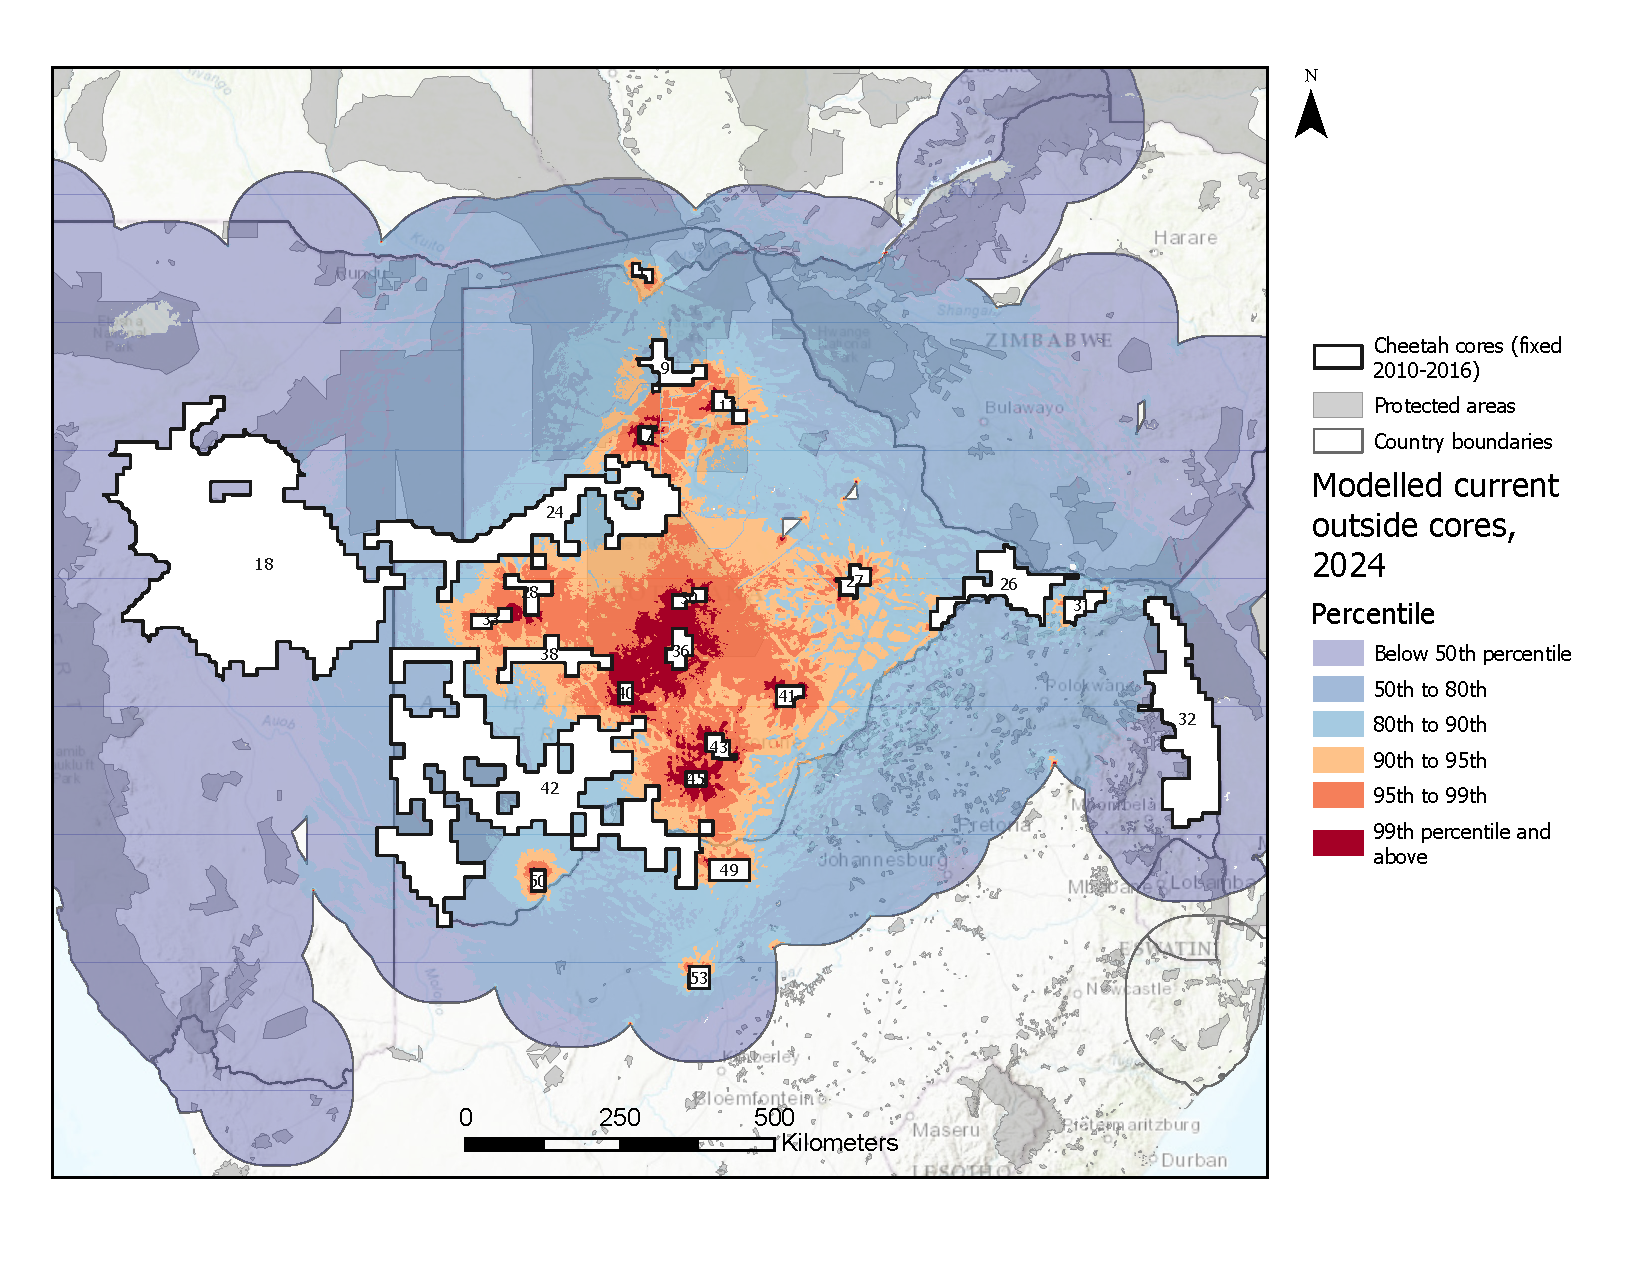
\includegraphics[width=\textwidth]{Figure_2A_modelled_current_2024.pdf}
  \caption{Modeled current concentration for 2024, with the fixed core network shown
  for orientation.}
  \label{fig:current2024}
\end{figure}
\FloatBarrier

\begin{table}[htbp]\centering
  \caption{Covariates, native resolution, source years, and static/dynamic treatment.}
  \label{tab:covariates}
  \small\begin{tabular}{>{\raggedright\arraybackslash}p{0.22\textwidth}>{\raggedright\arraybackslash}p{0.24\textwidth}>{\raggedright\arraybackslash}p{0.13\textwidth}>{\raggedright\arraybackslash}p{0.34\textwidth}}
\toprule
Covariate & Source & Treatment & Temporal role / notes\\
\midrule
Built-up fraction & Global Human Settlement Layer (GHSL) & Dynamic & 2010, 2015, 2020, 2025 products matched to snapshots\\
Nighttime radiance & Visible Infrared Imaging Radiometer Suite (VIIRS), VNL V2 & Dynamic & 2013, 2016, 2020, 2024 products\\
Tree cover & Moderate Resolution Imaging Spectroradiometer (MODIS), MOD44B & Dynamic & Annual snapshot fields\\
Non-tree vegetation & Moderate Resolution Imaging Spectroradiometer (MODIS), MOD44B & Dynamic & Annual snapshot fields\\
Bare cover & Moderate Resolution Imaging Spectroradiometer (MODIS), MOD44B & Dynamic & Annual snapshot fields\\
Road density & Global Roads Inventory Project, version 4 (GRIP4) & Static & Spatial pressure/context\\
Livestock density & Gridded Livestock of the World, version 4 (GLW4) & Static & Combined cattle, goats, and sheep exposure\\
Terrain / slope & Shuttle Radar Topography Mission (SRTM) & Static & Slope-derived resistance\\
Hydrography & Hydrological data and maps based on Shuttle Elevation Derivatives at multiple Scales (HydroSHEDS) & Static & Water/context mask\\
Veterinary fences & World Wide Fund for Nature (WWF), Kavango--Zambezi Transfrontier Conservation Area (KAZA); Kruger references & Scenario & Sensitivity/context, not assumed impassable\\
\bottomrule
\end{tabular}
\\[0.5em]
\parbox{\textwidth}{\footnotesize\emph{Note:} Product shorthand retained in the source names is defined at first use: VNL = VIIRS nighttime lights; V2 = product version 2; MOD44B = MODIS vegetation-continuous-fields product.}
\\[0.5em]
\noindent\TODO{THREE GAPS IN THIS TABLE, in plain terms.\\
1. The reader cannot tell which layers actually went into the resistance surface. Your final model used built-up, roads, livestock, and nighttime lights (human pressure), vegetation, and slope. Hydrography is listed as ``Water/context mask,'' but it was not one of the weighted inputs. Add a column or a note saying ``in resistance: yes/no'' so nobody assumes water was a barrier.\\
2. Categorical land cover (MCD12Q1) is not listed, but Methods says it was used for masking and description. Add it as ``Context only, never differenced.''\\
3. Protected areas (WDPA, August 2026) are not listed, but they drive a whole Results section. Add them as ``Overlay for reporting only, not a resistance input.''}

\end{table}

\begin{table}[htbp]\centering
  \caption{Ten highest-ranked modeled priority links shown from the 32-link primary-priority set.}
  \label{tab:top20}
  \resizebox{\textwidth}{!}{\begin{tabular}{rrrrrrr}
\toprule
From & To & Rank & Betweenness & Type & Distance (km) & Change (\%)\\
\midrule
38 & 40 & 1 & 0.409 & KNN+MST & 120.6 & +4.78\\
24 & 38 & 2 & 0.316 & KNN & 202.3 & +7.44\\
17 & 24 & 3 & 0.300 & KNN+MST & 208.0 & -5.78\\
30 & 40 & 4 & 0.238 & KNN & 169.2 & +3.55\\
27 & 41 & 5 & 0.103 & KNN+MST & 196.8 & -6.45\\
41 & 45 & 6 & 0.090 & KNN & 183.6 & -5.50\\
33 & 38 & 7 & 0.079 & KNN & 108.1 & +13.12\\
9 & 17 & 8 & 0.079 & KNN+MST & 109.0 & -5.26\\
26 & 27 & 9 & 0.079 & KNN+MST & 221.8 & -5.18\\
40 & 43 & 10 & 0.077 & KNN & 159.6 & -1.56\\
\bottomrule
\end{tabular}}
\parbox{\textwidth}{\footnotesize\emph{Note:} The table shows the ten highest-ranked members of the 32-link primary-priority set; links are modeled structural network relationships, not observed animal routes.}

\end{table}

\begin{table}[htbp]\centering
  \caption{Protected-area coverage of modeled high-current classes.}
  \label{tab:pa}
  \resizebox{\textwidth}{!}{\begin{tabular}{rrrrrr}
\toprule
Year & Current percentile & Cells & Protected (\%) & Background (\%) & Difference (pp)\\
\midrule
2012 & 80 & 418,295 & 24.23 & 31.26 & -7.03\\
2012 & 90 & 209,148 & 26.31 & 31.26 & -4.95\\
2012 & 95 & 104,574 & 35.57 & 31.26 & +4.31\\
2012 & 99 & 20,915 & 44.17 & 31.26 & +12.92\\
2024 & 80 & 418,292 & 23.27 & 31.26 & -7.99\\
2024 & 90 & 209,146 & 25.54 & 31.26 & -5.72\\
2024 & 95 & 104,573 & 33.45 & 31.26 & +2.19\\
2024 & 99 & 20,915 & 44.63 & 31.26 & +13.37\\
\bottomrule
\end{tabular}}
\\[0.5em]
\noindent\TODO{Final note: values use the outside-core, positive-current domain. Percentage-point differences are relative to the matched background. Do not report a permutation $p$-value because inference was sensitive to the assumed spatial block size.}

\end{table}

\begin{table}[htbp]\centering
  \caption{Overview of completed modeled-connectivity results.}
  \label{tab:priority}
  \begin{tabular}{p{0.53\textwidth}p{0.16\textwidth}p{0.25\textwidth}}
\toprule
Metric & Value & Interpretation\\
\midrule
Final modeled-current snapshots & 4 (2012, 2016, 2020, 2024) & 253/253 focal-region pairs connected each year\\
Fixed density cores & 23 & Historical baseline, fixed across snapshots\\
Selected neighboring links & 45 & Core-pair comparison set\\
Primary-priority links & 32 & Stable under weight/fence screens\\
All-pair median effective-resistance change & -1.224\% & 2012--2024\\
Selected-link median change & -1.557\% & 2012--2024\\
Primary-priority median change & -2.618\% & 2012--2024\\
Largest all-pair increase & +13.119\% & Link 33--38\\
Largest all-pair decrease & -8.243\% & Link 43--45\\
\bottomrule
\end{tabular}

\end{table}

\section{Discussion}
\label{sec:discussion}

\subsection{Connectivity change and comparison with previous work}
\TODO{PLAIN-LANGUAGE GUIDE: begin with the simplest overall result: the modeled ease
of moving between cores changed only slightly overall, but some individual links
changed more than others. Immediately state that the model describes landscape
structure and does not show where cheetahs actually moved.}

% Interpret individual increases and decreases in this same subsection.
\TODO{PLAIN-LANGUAGE GUIDE: describe where modeled connections became easier or
harder and which landscape changes occurred in the same places. Say "occurred in the
same places," not "caused." The model found mixed change rather than a broad decline.
Do not describe connectivity by country because core pairs were not assigned to
individual countries.}

% Compare these findings with previous regional studies here.
\TODO{PLAIN-LANGUAGE GUIDE: compare the general mapping approach with the elephant and
multi-species studies \parencite{naidoo2024kaza,brennan2020multispecies} and with the
fence study \parencite{osipova2018fencing}. Explain that similar mapping tools can be
used for different species, but the numerical resistance values cannot simply be
copied because each species responds differently to roads, vegetation, fences, and
people.}


\subsection{Protected areas and conservation context}
\TODO{PLAIN-LANGUAGE GUIDE: the strongest modeled concentrations often pass through
protected areas, but the wider land connecting those areas is less protected. Explain
that conservation therefore also depends on farms, communal lands, and other land
outside formal parks. This does not prove that protected areas failed. Also note that
parks are often located on land with lower agricultural value, which may partly shape
the pattern.}

\subsection{Priority links and field-survey needs}
\TODO{PLAIN-LANGUAGE GUIDE: links that stayed important under several assumptions are
the strongest candidates for conservation attention. Links that changed substantially
between assumptions are useful places for field surveys because better local data
could change the result. Agreement between scenarios is not complete proof because
the scenarios share many of the same input layers.}

% Survey implications follow directly from the uncertainty discussion.
\TODO{PLAIN-LANGUAGE GUIDE: there is no completed score that ranks individual survey
cells. Instead, explain how an organization could use the 13 uncertain links to choose
general survey areas, then adjust the order based on access, cost, safety, and local
knowledge. Link 17--24 is especially useful for checking because it is the only link
holding two parts of the three-neighbor network together, yet its mapped route was
highly unstable and had no overlap in 2020.}

\subsection{How far the tracking check supports the model}
\TODO{PLAIN-LANGUAGE GUIDE (UPDATED 5 OCTOBER 2026). One or two short paragraphs.\\
WHAT IT SHOWS: in one district, real free-ranging cheetahs moving from one day to the next tended to pick ground the model rates as easier than the ground they could have reached instead. This held for seven of nine animals and on all nine surfaces. A useful framing: the model passed a check it could have failed, because if the cats had picked higher-resistance ground, the result would have pointed the other way.\\
HOW BIG: modest. The real move beat about 56 percent of its alternatives, against 50 by chance. Call it a lean, not a match.\\
WHAT DRIVES IT: mostly roads. Road density alone did about as well as the full surface, and the cats crossed mapped roads less often than their alternative moves did. This fits work showing cheetahs avoid roads and busy areas (cite a source you already have, or add one). Be honest about the other side: vegetation on its own leaned slightly the wrong way, and modeled current showed no clear lean. Two possible reasons for the vegetation result, say them as possibilities, not findings: cheetahs in this ranchland may use denser bush for cover and hunting, and the tracks are older than the 2012 vegetation layer.\\
WHAT IT DOES NOT SHOW: that the model is right elsewhere (nine animals, one part of South Africa); anything about change over time (the tracks end in 2008); or anything about fences (none are mapped near the tracks, and the private game fences in this area are not in the model at all). Do not change any weight because of this check, and say you did not; using the tracks to tune the model would make the check no longer independent.\\
CLOSE WITH: the planned Namibia camera-trap comparison was not done, and independent movement data from fenced and more developed areas would be the most useful next test.}

\section{Limitations}
\label{sec:limitations}

% Write one paragraph containing no more than four sentences. Keep the detailed
% cautions in the supplement and project notes.

\TODO{SENTENCE 1: Say that the model shows where movement may be easier or harder,
but it does not prove where cheetahs actually traveled. SENTENCE 2: Say that the
cores and several landscape layers were kept constant through time, allowing a fair
comparison but limiting what could change between years. SENTENCE 3 (CORRECTED 5 OCTOBER 2026):
say that the resistance values were set by you, guided by published studies, and were
not fitted to cheetah movement data. The old prompt said they ``came from published
research,'' which overstates it, because the weights, the slope ramp, and the fence
multiplier were your choices. In the same sentence, say that rainfall was not checked,
so some vegetation change may reflect wet or dry years rather than land use, and that
source years did not always match the snapshot years. SENTENCE 4: Say that the mapped
paths are broad planning areas rather than exact travel routes, that the only
independent check came from nine animals in one district before 2012, and that the
results should be tested before use at another scale or in another region.}

\section{Conclusion}
\label{sec:conclusion}
% Sentence starters: "This study found that ..." / "The most robust priorities were ..." / "The practical recommendation is ..." / "Overall, these results describe ... rather than ..."
\TODO{PLAIN-LANGUAGE GUIDE: use only three or four sentences. First, say that modeled
connectivity changed only slightly overall and that individual links changed in both
directions. Second, say that the strongest concentrations often reached protected
areas but the wider connecting landscape was less protected. Third, state that 32
links were retained as main priorities and 13 were identified as places needing more
field information. End by reminding the reader that these are modeled landscape
connections, not observed cheetah routes. Do not add new results here.}


\ifcapstone
  \section*{Data availability}
\addcontentsline{toc}{section}{Data availability}
\TODO{PLAIN-LANGUAGE GUIDE: add the final repository or archive link and DOI. State
that the scripts and outputs created by the project are available there. Explain that
raw protected-area data must be downloaded from Protected Planet under its license and
that cheetah occurrence locations can only be shared at the detail allowed by their
source.}

\section*{Acknowledgements}
\addcontentsline{toc}{section}{Acknowledgements}
\TODO{PLAIN-LANGUAGE GUIDE: list the department, advisor, data providers, and any
organization or person who reviewed the project or helped interpret priorities.}

\section*{Funding}
\addcontentsline{toc}{section}{Funding}
\TODO{LANDSCAPE ECOLOGY REQUIRES THIS STATEMENT. If nobody paid for the work, Springer's own wording is: ``The authors did not receive support from any organization for the submitted work.'' If a scholarship, department, or grant helped, name it and give any grant number.}

\section*{Conflicts of interest}
\TODO{Springer calls this heading ``Competing interests''. Rename it when you submit.}
\addcontentsline{toc}{section}{Conflicts of interest}
I declare no conflicts of interest.

  \printbibliography
\else
  % Springer order: references, then the required statements under one
  % heading, each statement as a subheading.
  \printbibliography
  \section*{Statements and Declarations}
  \begingroup
    \let\section\subsection
    \section*{Data availability}
\addcontentsline{toc}{section}{Data availability}
\TODO{PLAIN-LANGUAGE GUIDE: add the final repository or archive link and DOI. State
that the scripts and outputs created by the project are available there. Explain that
raw protected-area data must be downloaded from Protected Planet under its license and
that cheetah occurrence locations can only be shared at the detail allowed by their
source.}

\section*{Acknowledgements}
\addcontentsline{toc}{section}{Acknowledgements}
\TODO{PLAIN-LANGUAGE GUIDE: list the department, advisor, data providers, and any
organization or person who reviewed the project or helped interpret priorities.}

\section*{Funding}
\addcontentsline{toc}{section}{Funding}
\TODO{LANDSCAPE ECOLOGY REQUIRES THIS STATEMENT. If nobody paid for the work, Springer's own wording is: ``The authors did not receive support from any organization for the submitted work.'' If a scholarship, department, or grant helped, name it and give any grant number.}

\section*{Conflicts of interest}
\TODO{Springer calls this heading ``Competing interests''. Rename it when you submit.}
\addcontentsline{toc}{section}{Conflicts of interest}
I declare no conflicts of interest.

  \endgroup
\fi

\appendix
\section{Analysis protocol as predeclared}
\label{app:protocol}
\TODO{FOR BIODIVERSITY AND CONSERVATION: this appendix is not part of the submitted manuscript. It becomes a separate file, Online Resource 1, uploaded as \texttt{ESM\_1.pdf}. Springer asks that every supplementary file include, at the top, the article title, journal name, author names, and the corresponding author's affiliation and email, plus a short caption describing the file. In the main text it is referred to as ``Online Resource 1''; typing \texttt{\textbackslash suppA} prints that automatically in the submission layout and ``Appendix A'' in the capstone.}
\TODO{PLAIN-LANGUAGE GUIDE FOR THE PROTOCOL APPENDIX.
The saved protocol is tagged \texttt{protocol-v1.0} in the
\texttt{cheetah-connectivity} repository at commit
\texttt{d7de8675a074dfbffc0c7c856bb5645e1e13867d}, dated 18 August 2026. However, the
file itself still says version 0.1 draft. Do not change the old file. Explain that the
Git tag marked the saved version even though its internal label was not updated.
Then list, in simple terms, what changed between the plan and the final analysis: the
core definition, sensitivity tests, definition of a stable link, scenario names,
network measurements, protected-area comparison, monitoring index
that was not built, and 2030 scenarios that were added later. Include the objective
and hypothesis outcomes: O1 was completed; O2 was narrowed; O3 was replaced rather
than completed; H1 was mixed; H2 did not pass its full rule; H3 was only partly tested
and did not match the ``limited subset'' prediction; and H4 was not tested.}

\TODO{ADDED 5 OCTOBER 2026: FOUR MORE ITEMS FOR THE CHANGE LIST, plus one correction.\\
1. A MAIN SURFACE WAS CHOSEN. The protocol said no resistance scenario would be treated as the main answer. The paper uses the vegetation-balanced surface with documented fences as the main one and reports the rest as sensitivity. Say this was a change and give your reason in one sentence.\\
2. WHEN THE WEIGHTS WERE SET. Say plainly whether the final weights (60/20/20 and 30/30/30/10) were fixed before or after you had looked at resistance maps or results. This is the first thing a reader checks in a predeclared study. Either answer is acceptable if it is stated honestly; if any weight was adjusted after seeing outputs, say which one and why.\\
3. PC/dPC WAS DROPPED. The protocol planned probability of connectivity at 50, 100, 200, and 400~km. Only betweenness was calculated. Give the real reason (see the TODO in the Network structure subsection).\\
4. ONE CORE DEFINITION, NOT THREE. The protocol planned three core definitions with minimum areas of 2,000, 1,000, and 500~km$^2$. The analysis used one density-based definition. List it here if it is not already covered by ``core definition'' above.\\
CORRECTION: the old list included ``occurrence check'' as a change. That is no longer true. The planned independent tracking check (protocol steps 23.1--23.5) was completed using the Limpopo data. What is still different from the plan: the Namibia camera-trap comparison was not done, and two kinds of analysis were added. First, a second, same-archive occurrence check. Second, four stricter follow-ups to the tracking check (a step check comparing each real move with moves the animal could have made instead, a breakdown by input layer, a repeat on all nine surfaces, and a road-crossing count). List these as additions, say they were added after the planned check was run, and say that none of them changed any weight or the choice of main surface.}

\section{Supplementary material}
\label{app:supplement}
\TODO{FOR BIODIVERSITY AND CONSERVATION: this becomes Online Resource 2, uploaded as \texttt{ESM\_2.pdf}, with the same header details as Online Resource 1 (article title, journal name, author names, corresponding author's affiliation and email). Number its tables S1, S2, and so on, and refer to them in the main text as, for example, ``Online Resource 2, Table S4''; \texttt{\textbackslash suppB} prints the ``Online Resource 2'' part.}
\TODO{PLAIN-LANGUAGE GUIDE: the tables below preserve details that are useful for
checking the analysis but are too long for the main paper. They cover which source year
matched each modeled year, strongly related predictors, overlap of high-current areas,
software versions, vegetation assumptions, route stability, and the 2030 scenarios.
Do not add tables for different map resolutions or a cell-level monitoring score
because those analyses were not completed.}

\begin{table}[htbp]\centering
  \caption{\TODO{Final caption: software environment used for the completed analysis.}}
  \label{tab:software}
  \begin{tabular}{lll}
\toprule
Component & Version & Verification\\
\midrule
ArcGIS Pro & 3.7.2 (build 1901) & \texttt{arcpy.GetInstallInfo()}\\
ArcGIS Python & 3.13.13 & ArcGIS Pro environment\\
Julia & 1.12.7 & \texttt{julia --version}\\
Circuitscape.jl & 5.17.1 & Julia package environment\\
Google Earth Engine & Cloud service & Acquisition and harmonisation\\
\bottomrule
\end{tabular}

\end{table}

\begin{table}[htbp]\centering
  \caption{\TODO{Final caption: temporal matching of dynamic covariates to the four analysis snapshots.}}
  \label{tab:temporal-alignment}
  \resizebox{\textwidth}{!}{\begin{tabular}{lllllll}
\toprule
Covariate & Source & Treatment & 2012 snapshot & 2016 snapshot & 2020 snapshot & 2024 snapshot\\
\midrule
Built-up fraction & GHSL & Dynamic & 2010 ($-2$) & 2015 ($-1$) & 2020 (0) & 2025 ($+1$)\\
Nighttime radiance & VIIRS VNL V2 & Dynamic & 2013 ($+1$) & 2016 (0) & 2020 (0) & 2024 (0)\\
Tree cover & MODIS MOD44B C6.1 & Dynamic & 2012 (0) & 2016 (0) & 2020 (0) & 2024 (0)\\
Non-tree vegetation & MODIS MOD44B C6.1 & Dynamic & 2012 (0) & 2016 (0) & 2020 (0) & 2024 (0)\\
Bare ground & MODIS MOD44B C6.1 & Dynamic & 2012 (0) & 2016 (0) & 2020 (0) & 2024 (0)\\
Land cover & MODIS MCD12Q1 C6.1 & Context only & 2012 (0) & 2016 (0) & 2020 (0) & 2024 (0)\\
\bottomrule
\end{tabular}}
\\[0.5em]
\noindent\TODO{Final note: values in parentheses are source-year minus nominal-year offsets. Define GHSL, VIIRS, VNL, and MODIS here.\\
MISSING ROW: the source CSV has a rainfall row (CHIRPS annual precipitation) marked ``not yet acquired.'' The table leaves it out, which hides that the rainfall check was never done. Your Limitations prompt already mentions rainfall. Pick one: add the row back and say ``planned, not completed,'' or keep it out and make sure the Limitations sentence says plainly that rainfall was not checked. Either is fine; just do not leave it silent, because vegetation change can come from a wet or dry year rather than from land use.}

\end{table}

\begin{table}[htbp]\centering
  \caption{\TODO{Final caption: predictor pairs with absolute Spearman correlation of at least 0.75.}}
  \label{tab:predictor-correlation}
  \begin{tabular}{lr}
\toprule
Predictor pair & Spearman $\rho$\\
\midrule
Tree cover--bare ground & $-0.877$\\
Non-tree vegetation--bare ground & $-0.836$\\
Cattle--goats & $0.774$\\
\bottomrule
\end{tabular}
\\[0.5em]
\noindent\TODO{Final note: report only pairs with $|\rho| \geq 0.75$ from the archived 2024 predictor screen.}

\end{table}

\begin{table}[htbp]\centering
  \caption{\TODO{Final caption: pairwise overlap of outside-core high-current cells among successive snapshots and endpoints.}}
  \label{tab:current-overlap}
  \begin{tabular}{rrrrrrr}
\toprule
Earlier year & Later year & Earlier cells & Later cells & Intersection & Union & Jaccard\\
\midrule
2012 & 2016 & 209,148 & 209,150 & 200,069 & 218,229 & 0.917\\
2016 & 2020 & 209,150 & 209,147 & 201,179 & 217,118 & 0.927\\
2020 & 2024 & 209,147 & 209,146 & 199,881 & 218,412 & 0.915\\
2012 & 2024 & 209,148 & 209,146 & 199,511 & 218,783 & 0.912\\
\bottomrule
\end{tabular}
\\[0.5em]
\noindent\TODO{Final note: cells are the outside-core top decile of positive modeled current in each snapshot.}

\end{table}

\begin{table}[htbp]\centering
  \caption{\TODO{Final caption: conditional 2030 scenario changes in selected-link least-cost path cost relative to 2024.}}
  \label{tab:future2030}
  \begin{tabular}{lrrrr}
\toprule
Scenario & Links & Median change (\%) & Minimum (\%) & Maximum (\%)\\
\midrule
2024 held constant (reference) & 45 & 0.00 & 0.00 & 0.00\\
Half of the 2012--2024 trend extended & 45 & $-3.36$ & $-8.53$ & $+6.06$\\
Full 2012--2024 trend extended & 45 & $-6.94$ & $-17.12$ & $+8.65$\\
\bottomrule
\end{tabular}
\\[0.5em]
\noindent\TODO{Final note, in your own words. Change is relative to the 2024 surface.
Only built-up area and vegetation (tree, non-tree, bare) were pushed forward along their
2012--2024 straight-line trend; nighttime lights, roads, livestock, terrain, fences, and
the cores were held at 2024. These are ``what if the recent trend kept going'' tests, not
forecasts.\\
WHY THE ROWS WERE RENAMED: they used to say ``Low growth,'' ``Continuation,'' and ``High
development.'' Those names were misleading. The ``low growth'' row is zero by
construction because nothing changed. The ``high development'' row extends the whole
trend, and that includes vegetation. Vegetation made links easier from 2012 to 2024, so
extending it makes links easier still ($-6.94\%$). A reader who sees ``high development''
expects connections to get harder, so the old label would look like a mistake.\\
WHAT TO SAY ABOUT IT: one sentence noting that the projected change is mostly driven by
the vegetation trend, not by new development. If you want a true ``more development''
test, it would need built-up and lights pushed forward with vegetation held at 2024;
that run does not exist yet.}

\end{table}

\begin{table}[htbp]\centering
  \caption{\TODO{Final caption: sensitivity of 2012--2024 selected-link cost change to vegetation weighting.}}
  \label{tab:vegetation-sensitivity}
  \begin{tabular}{lrr}
\toprule
Vegetation weighting & Links & Median absolute change (\%)\\
\midrule
Low & 45 & 3.57\\
Balanced & 45 & 6.27\\
High & 45 & 9.28\\
\bottomrule
\end{tabular}
\\[0.5em]
\noindent\TODO{Final note: 43 of 45 links retained the same 2012--2024 change direction under all three vegetation weightings.}

\end{table}

\begin{table}[htbp]\centering
  \caption{\TODO{Final caption: route-location sensitivity under the corrected vegetation inputs.}}
  \label{tab:route-location-sensitivity}
  \begin{tabular}{lrrrr}
\toprule
Link set & Links & Route-years & Route-years below 80\% & Affected links\\
\midrule
All selected links & 45 & 180 & 49 & 29\\
Primary-priority links & 32 & 128 & 34 & 21\\
\bottomrule
\end{tabular}
\\[0.5em]
\noindent\TODO{Final note: the threshold requires at least 80 percent reciprocal route overlap within 1 km; it is a sensitivity screen, not a biological cutoff.}

\end{table}

\TODO{PLAIN-LANGUAGE DATA CHECK: every value in these tables should come from a CSV in
\texttt{tables/source\_data/}. Never copy a number from a screenshot or estimate it
from a map legend.}

\begin{figure}[p]\centering
  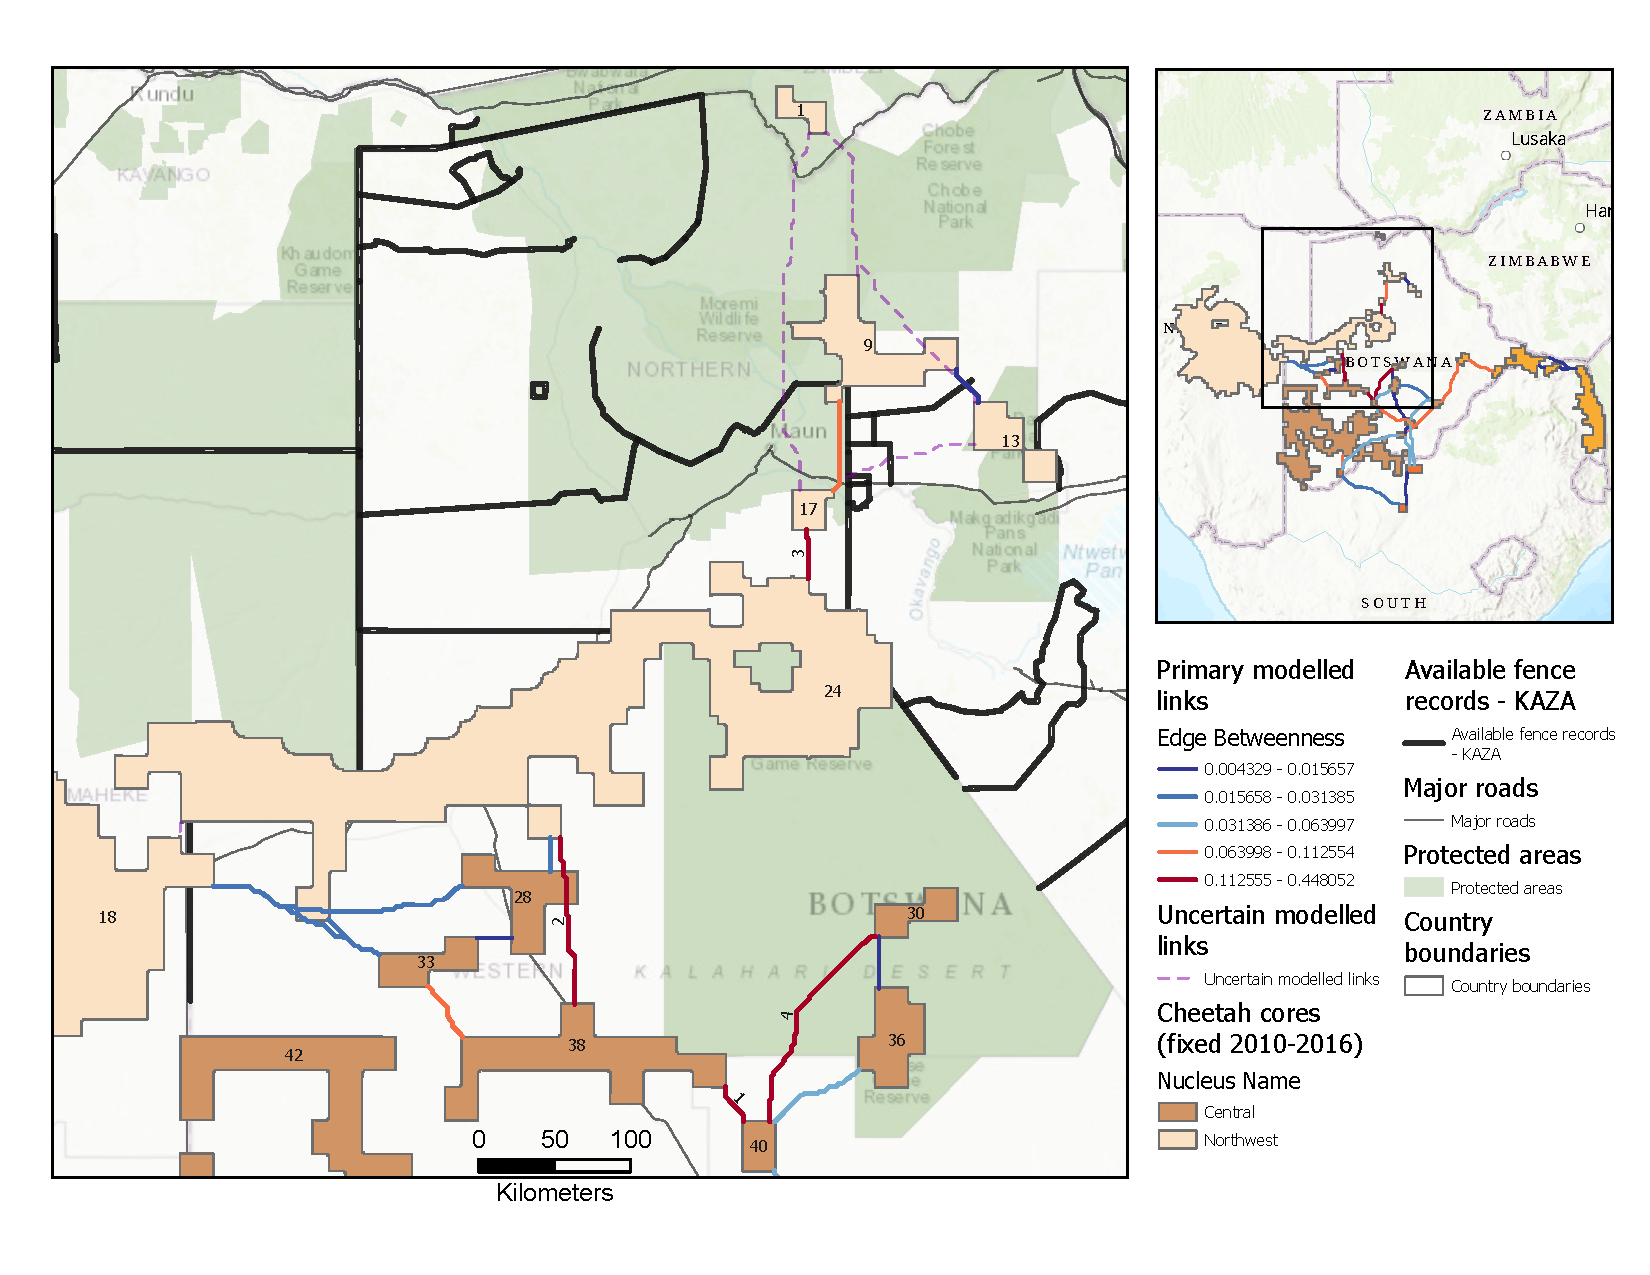
\includegraphics[width=0.48\textwidth]{Supplement_northwest_detail.pdf}\hfill
  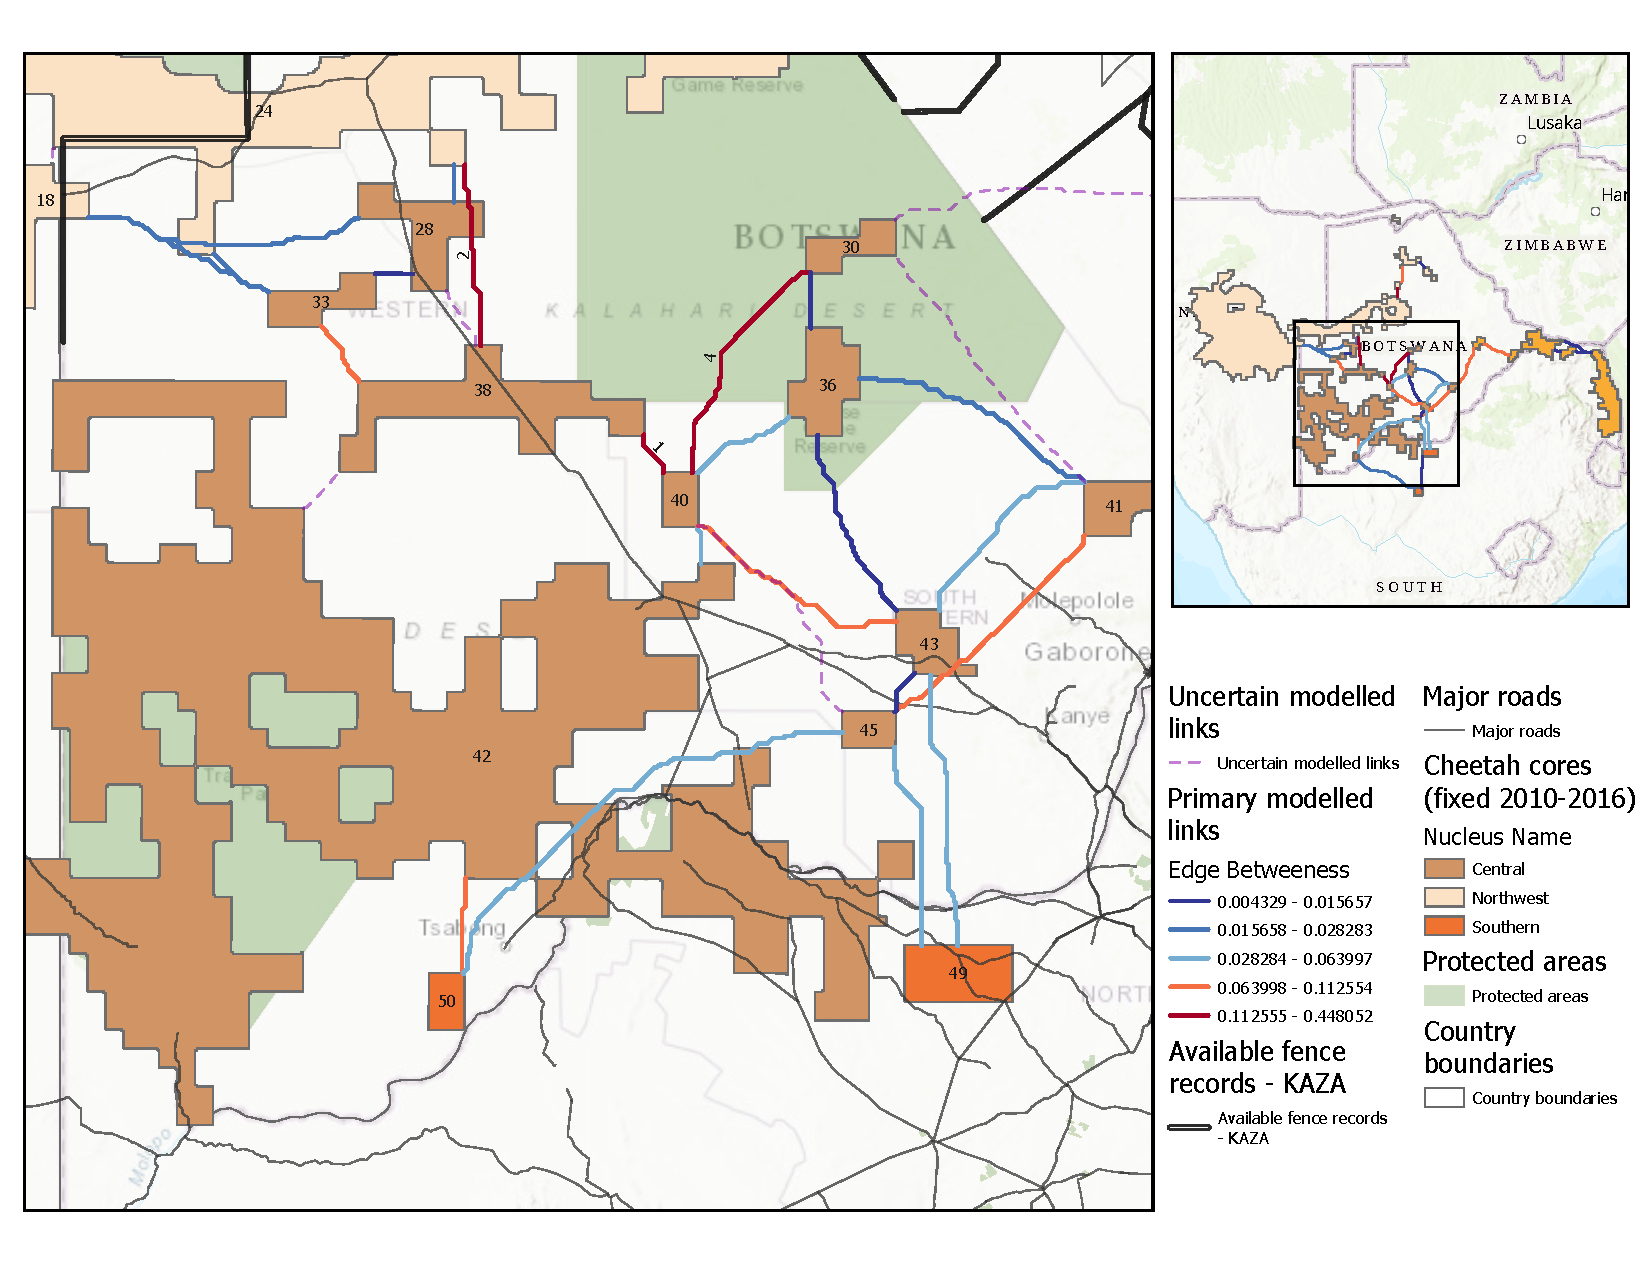
\includegraphics[width=0.48\textwidth]{Supplement_central_detail.pdf}\\[0.75em]
  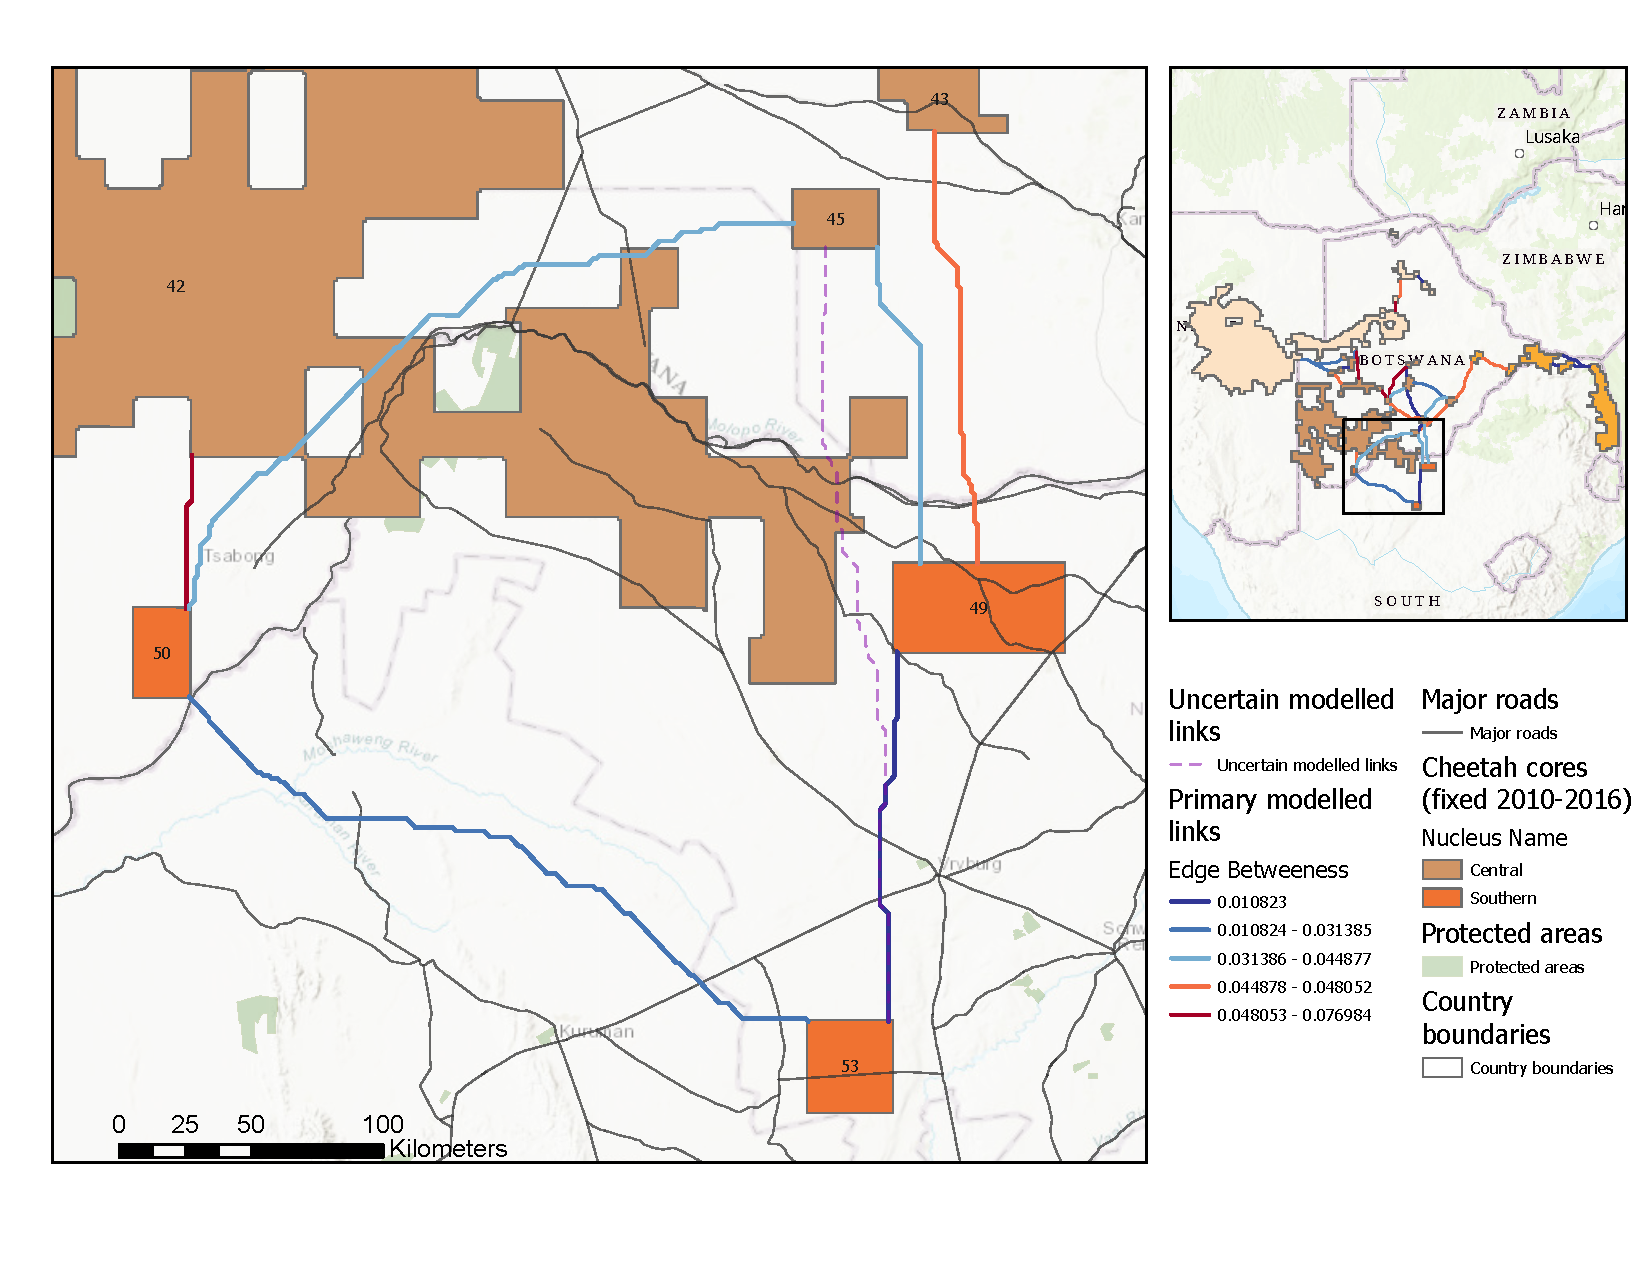
\includegraphics[width=0.48\textwidth]{Supplement_southern_detail.pdf}\hfill
  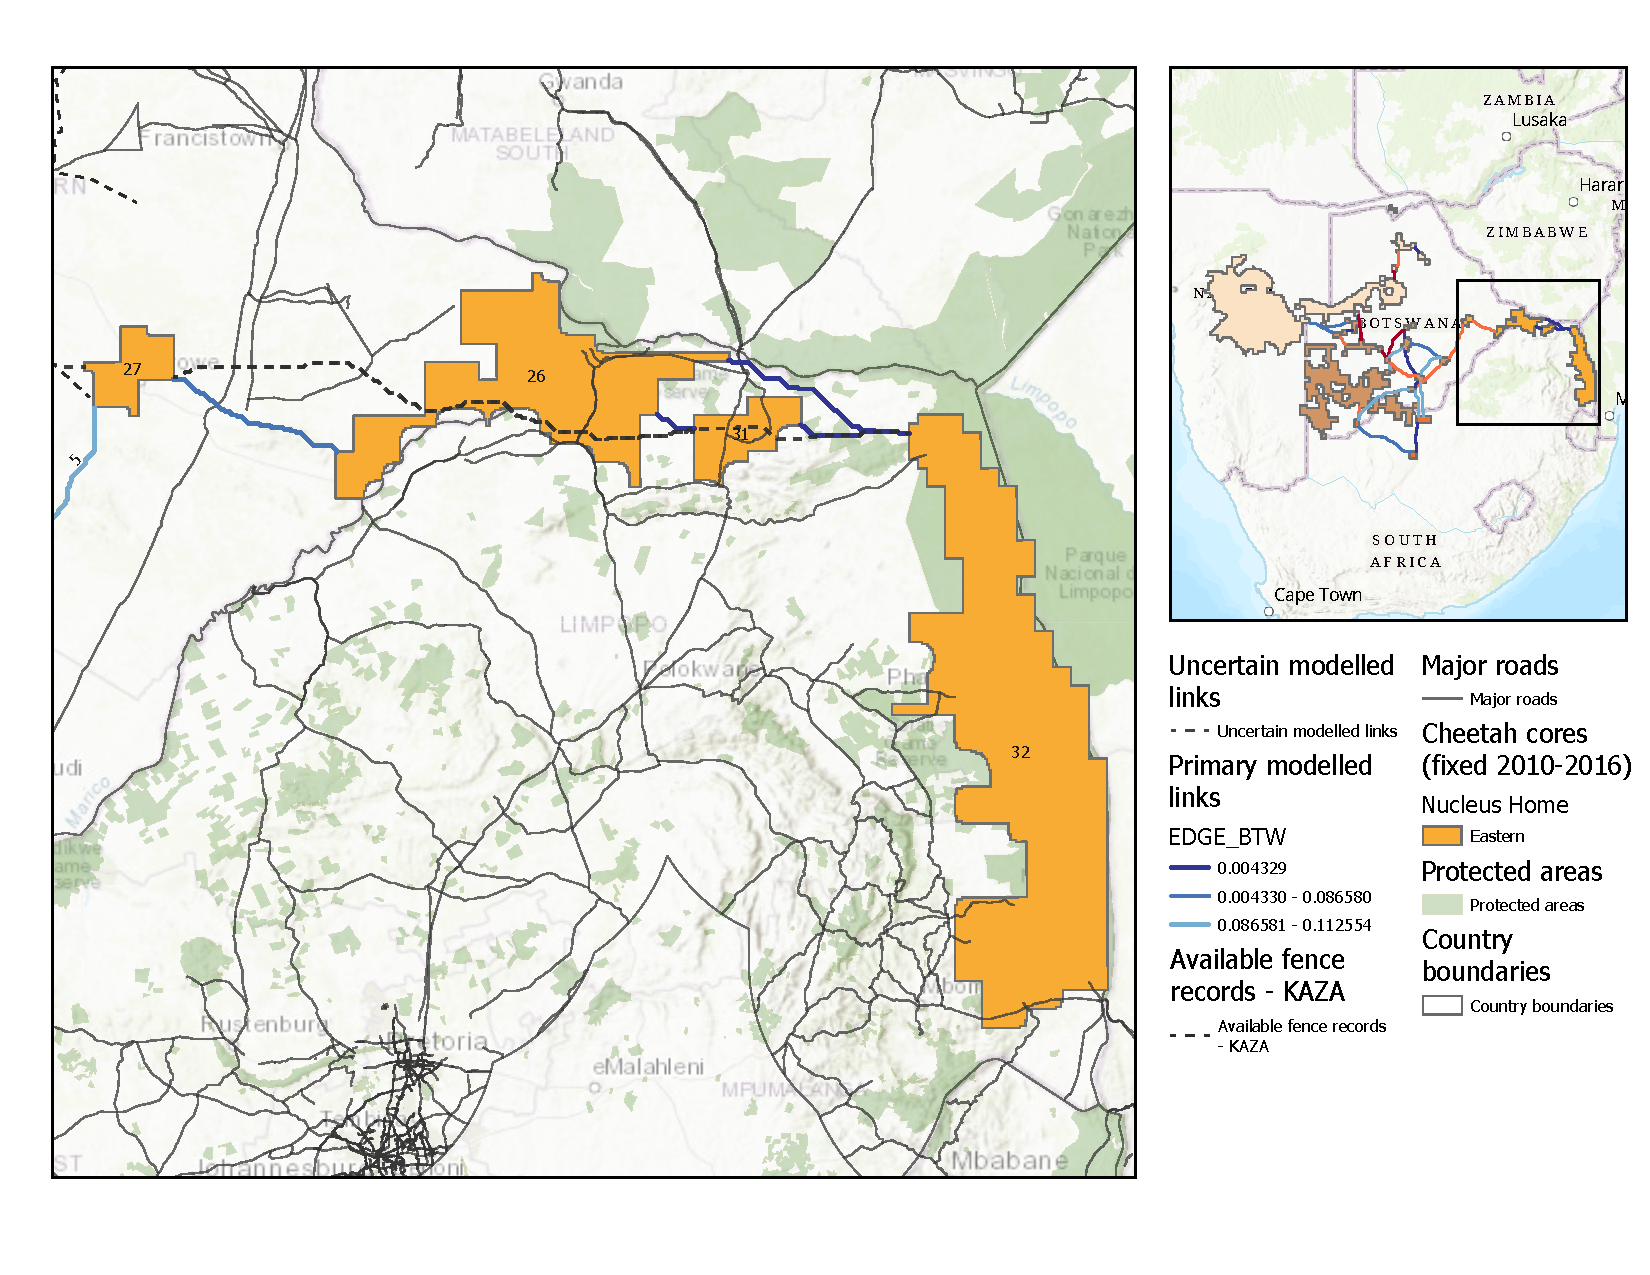
\includegraphics[width=0.48\textwidth]{Supplement_eastern_detail.pdf}
  \caption{Regional detail maps corresponding to the modeled-link network. These
  panels support visual inspection of local context and are supplementary to the
  main network and priority-link figures.}
  \label{fig:regionaldetails}
\end{figure}


\end{document}
